\documentclass[a4, 12 pt]{article} % delete two column for single column reports
\usepackage{graphicx}
\usepackage{amsmath}
\usepackage{caption}
\usepackage{nomencl}
\usepackage{array}
\usepackage{amssymb}
\usepackage{xfrac}
\captionsetup[figure]{labelfont=bf}
\captionsetup[table]{labelfont=bf}
\usepackage{tocloft}
\usepackage{float}
\setcounter{tocdepth}{4}
\setcounter{secnumdepth}{4}
\renewcommand{\thesection}{\arabic{section}}
\usepackage{titlesec}
\usepackage{lipsum}
\usepackage{appendix}
\usepackage{authblk}

%CHANGE INDENTATION HERE
\usepackage[top=1.2in, bottom=1.2in, left=1in, right=1in]{geometry}
\usepackage{fancyhdr}
\pagestyle{fancy}
\usepackage{sectsty}
\sectionfont{\fontsize{12}{16}\selectfont}
\subsectionfont{\fontsize{12}{14}\selectfont}
\usepackage[export]{adjustbox}
\begin{document}
\begin{titlepage}
\newcommand{\HRule}{\rule{\linewidth}{0.5mm}} 
\centering

%INSERT TITLE, AUTHORS & SUBTITLE HERE
\textsc{\Large Science Payloads and Advanced Concepts for Exploration (SPACE) Interactive Tool \\[7mm] \normalsize Zoe Himwich, Aparna Natarajan, Huong Vo\\[4mm] Mentor: Dr. Pamela E. Clark}\\[0.8cm] 
\textsc{NASA Goddard Space Flight Center, Greenbelt, Maryland}\\[124mm] 

%INSERT LOGOS HERE, MAKE SURE FILES ARE IN WORKING DIRECTORY
\begin{figure}[h]
\centering
\begin{minipage}{.5\textwidth}
  \centering
  
\includegraphics[width=1\linewidth, left]{goddard.jpg} %rename
\end{minipage}%
\begin{minipage}{.5\textwidth}
  
\includegraphics[width=0.55\linewidth, right]{nasa.png} %rename
\end{minipage}
\end{figure}
\end{titlepage}

%UNCOMMENT FOR TABLE OF CONTENTS
\tableofcontents
\newpage

%INSERT ABSTRACT HERE

%The abstract should provide a brief overview of the report.  It should provide a summary of the main specific points for the introduction, the main tests and experiments, the results, and the conclusions. It is called an abstract because you can literally "abstract" sentences from the other sections. Once again, this is not a narrative of your experiences as you executed the design.  The abstract should mirror (albeit in a very condensed way) the content of your report.
\begin{abstract}
Here at Goddard Space Flight Center, we have developed an online CubeSat design tool, geared towards deep space exploration based on a specific mission requirement -- henceforth referred to as the SPACE tool. The tool is ideal for scientists and engineers who wants to draw up a complete, but preliminary system, consisting of parts that are a mixture of commercial off the shelf, as well as research innovations -- making the overall cost much more manageable. SPACE walks the user through a series of questions and forms, eventually parsing these parts together for a final design consisting of seven separate subsystems. We hope that with the development of this tool, we can eventually move towards a standardization of the CubeSat paradigm, making it cheaper, faster, and easier than ever to design a CubeSat. 
%
%that allows scientists who want a low budget spaceflight mission to draw up early designs for a CubeSat. CubeSats are small satellites, typically with a volume less than or equal to 1200cm3. CubeSats only have room for one science instrument, but their small size makes them ideal for low cost, single purpose missions.
%The tool selects parts for a CubeSat based on user inputs. It divides a standard CubeSat into seven subsystems; instrument, attitude control system, propulsion, data handling and computing, power, frame, and
%communication. Each page of the site guides the user through a different subsystem.
%
%Provides a basic system for a deep space CubeSat based off of user specifications for a mission.


\end{abstract}

%BODY OF LAB REPORT

%Brief introduction and overview of the purpose of the project and of the methods and tools used.  the introduction should elaborate the abstract
\section{INTRODUCTION}
CubeSats are small satellites grouped under the umbrella category of nano-satellites, coming in units that are each 10 cm x 10 cm x 10 cm, weighing about 1.33 kg. A CubeSat can, and often, consists of multiple units of various configurations depending on the mission requirements. It was first introduced in 1999, by Bob Twigs (Stanford) and Jordi Purig-Surai (Cal Poly), in order to allow graduate students to develop and test small, low cost spacecraft in low earth orbit. Since then, the idea of miniature, economical spacecraft has become increasingly popular, propagating CubeSat development as well as the miniaturization of existing technologies all throughout the professional market.  \\[3mm]
While CubeSats have become very ubiquitous and economically sustainable within low-earth orbit, they are not being utilized to their full potentials -- i.e., beyond the low-earth orbit. We feel that this is the logical next step, based on several different facets of the CubeSat paradigm. First and foremost, if we begin to use CubeSats for deep space science missions, we can obtain a dynamic view of the target through a multi-platform approach, instead of the current, static view we are able to achieve through the use of one conventional spacecraft. Furthermore,  CubeSats can be easily integrated as a secondary payload, with minimal expenditures. Its small form factor allows for a reduction of launch costs, and the standardization leads to a predictability that will reduce failure rates. With the SPACE Tool, we are encouraging the user to develop missions for targets much beyond LEO (although that will be an option), through introducing instrumentation and subsystems that were developed for use in a deep space environment.
\section{SUBSYTEMS}
The tool consists of a series of webpages, beginning with the instrumentation and ending with the thermal and mechanical subsystems. While SPACE can be used without a preconceived mission requirement, it is better to come in to the design process with some preliminary planning. This starts with the introduction page, which asks for a target planet that the user would like to fly by. Choosing this target will affect the calculations later on during the trajectory planning, as well as the communication path. Knowing the science requirement of the mission before starting this tool will also streamline the instrumentation selection process, the most crucial selection of the entire design process -- as the instrumentation is the core of every science-based CubeSat.\\[3mm]
That said, we have ensured to create a thoroughly documented website, so any new user will be able to come in and create a CubeSat using the technologies we have laid out for them. There are instructions and explanations on every page for the required inputs as well as some suggested range that have been used in the past, and before the user even start the tool, the landing page has a brief explanation of the algorithms we use to present the parts on each page. Every subsection uses the same method to add a part to the current design, which is responsive and straightforward, and the user will be able to go back and redesign as they wish. However, only when a page is completely filled out, can a user move forward -- this ensures no bugs are created in later calculations. The user will also be able to see a snapshot for their most up-to-date design on every page, as they are working. There is also an icon, with the letter i in it for each page next to the available parts window, which will let the user view more information about their desired part so they can make the choice best suited for their mission.  We will now proceed to describe each subpage in details, and present our methods of filtering down available parts.
\subsection{Mission Planning}
In this section, the user is asked to fill out some brief descriptors of their mission -- such as a name, an objective, as well as their target planet. The objective can be as brief or as detailed as the user wishes, and same goes for the name. The available targets for exploration are as follow: Earth (in low, medium, or high orbit), Mercury, Mars, Venus, and the Moon. There is a right arrow button next to each required fields, which the user can double click to add the inputs to the current design. The user will be able to progress to the next page, when all three fields are filled out and added to the CubeSat. One caveat: if the user chooses to go to the previous page, their CubeSat will be removed from the database and they will lose all their work. 
\begin{figure}[H]
\begin{center}
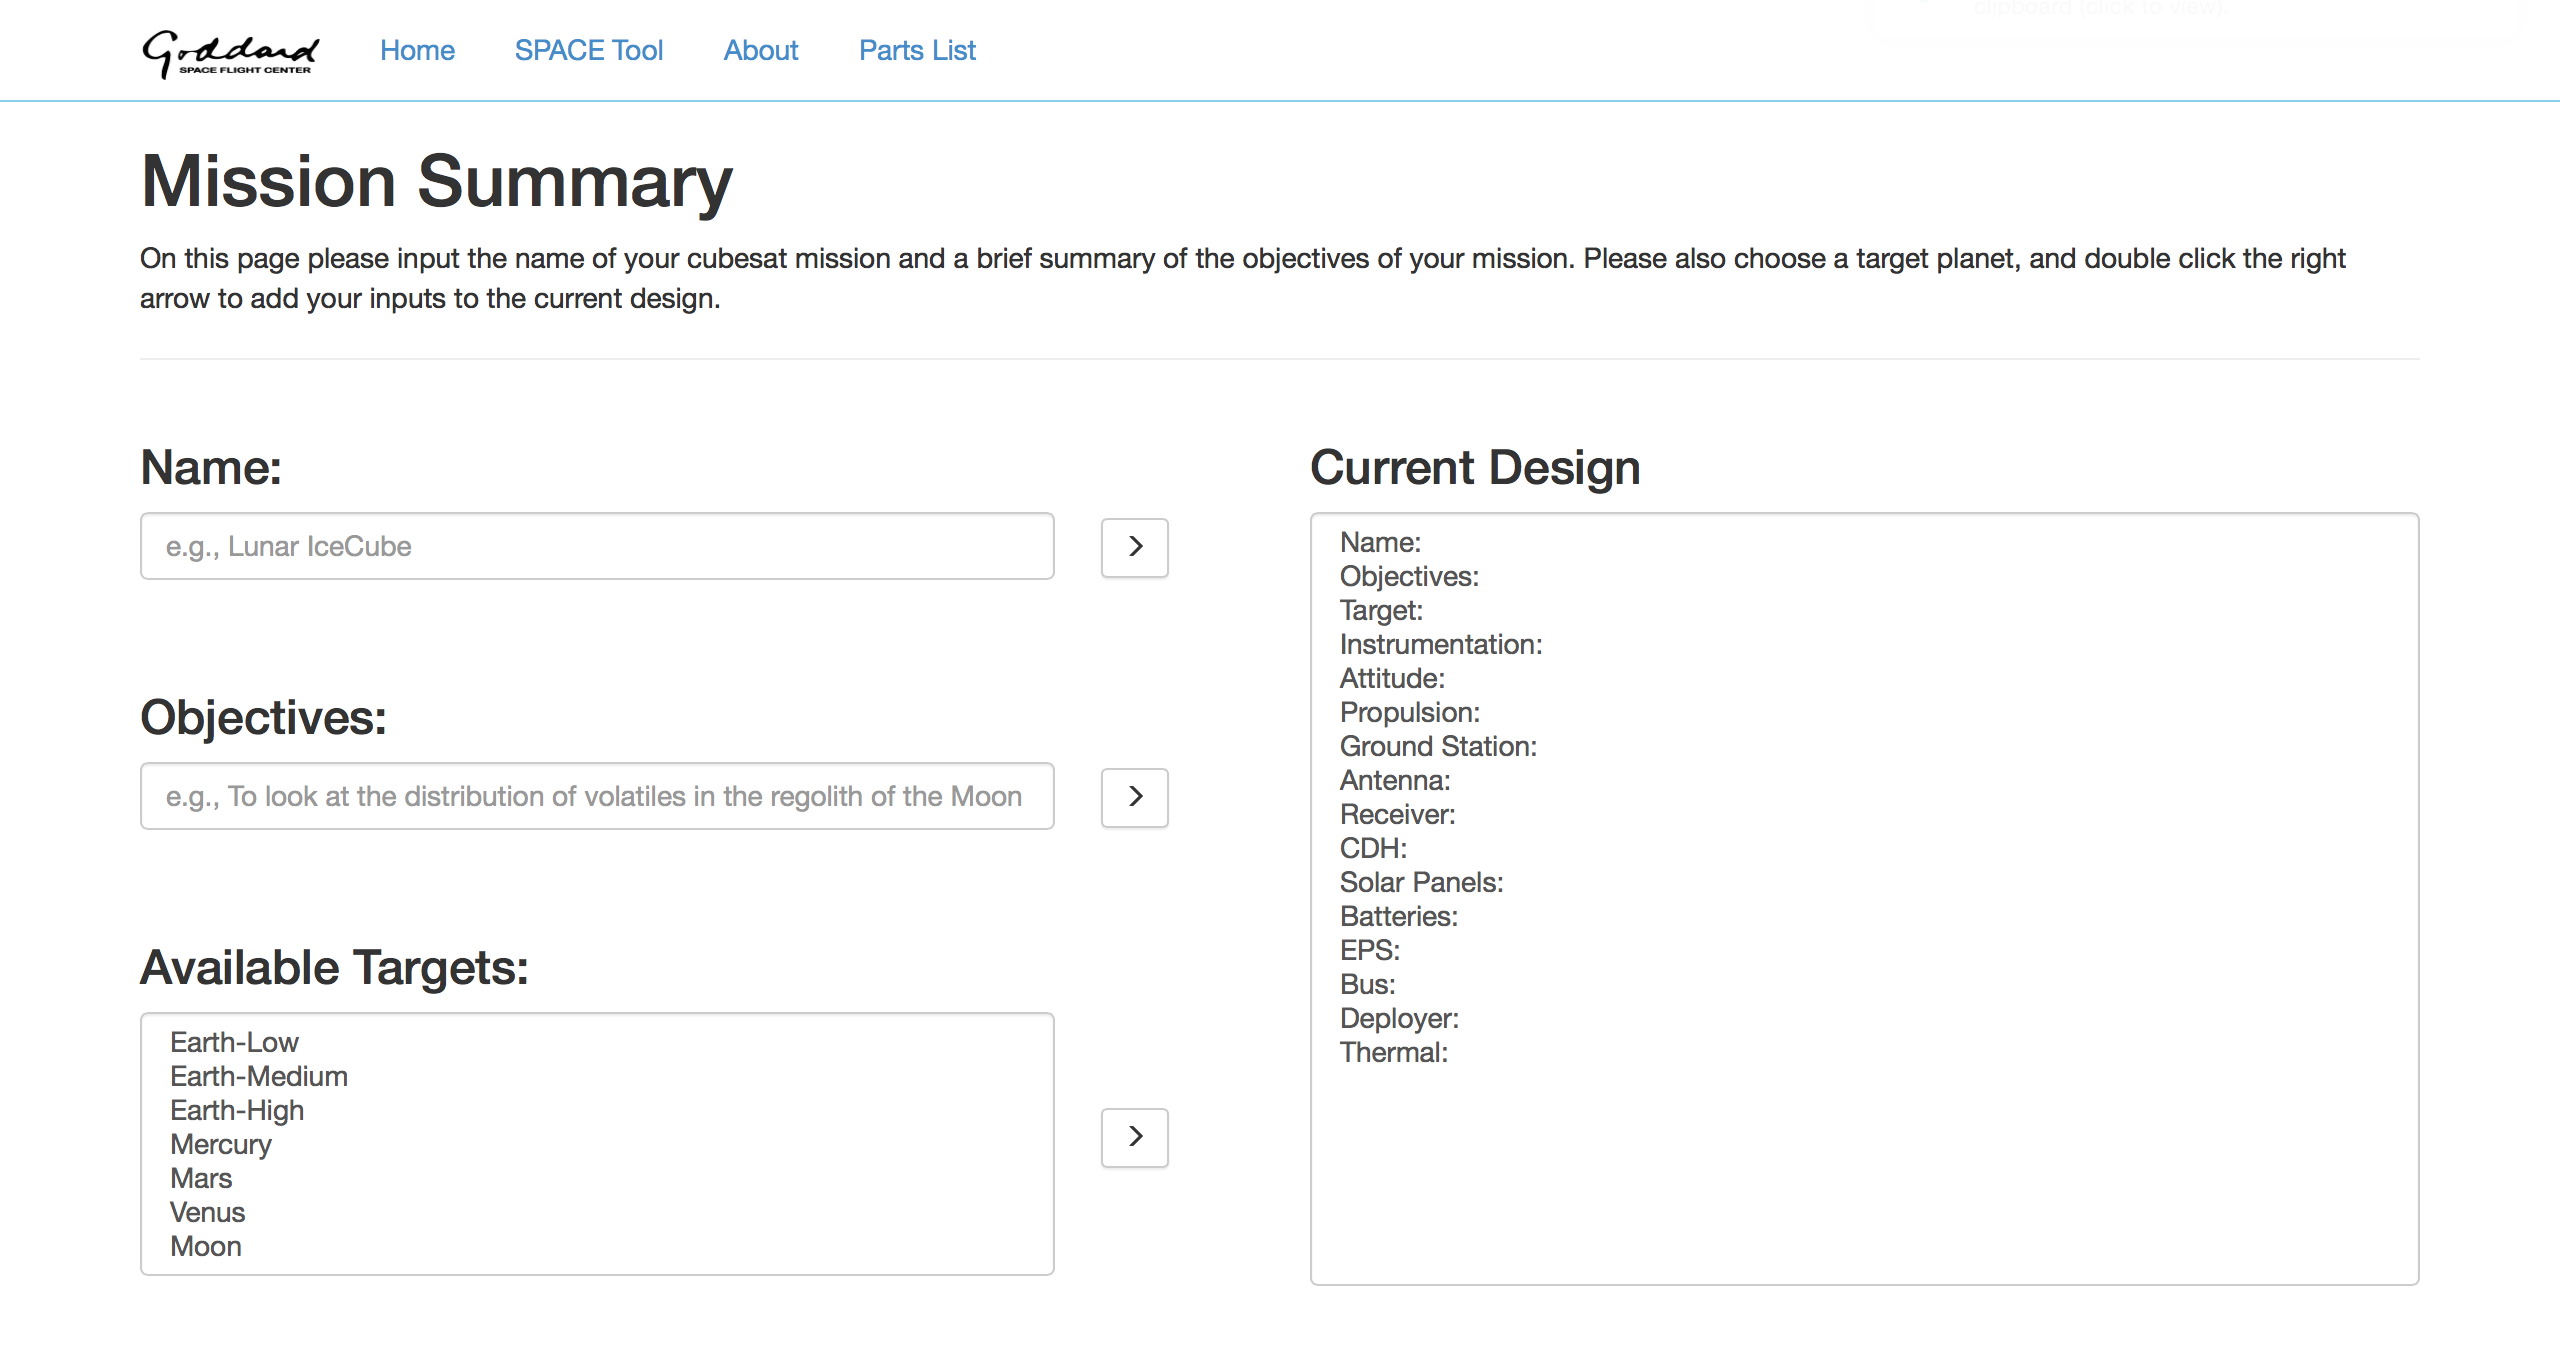
\includegraphics[width=\linewidth]{1}
\caption{Screenshot of the mission planning page}
\label{default}
\end{center}
\end{figure}

\subsection{Instrument Selection}
In this section, the user is asked to choose an instrumentation for their CubeSat. This section is crucial in the design process, as the instrumentation is what will carry out the science requirements. The selection is revolved around the electromagnetic spectrum -- based on the guiding principle that each part of the spectrum is governed by different energy production mechanisms, detection methods, as well as analysis technique associated. We have divided the spectrum into five separate sub-region, with detailed explanations of what each section can handle in terms of remote sensing. The general idea is that as the wavelengths increase, the scale of the natural processes occurring that can be looked at with the light increases, but so does the depth of penetration. It is recommended that the user at least knows the scale of their science requirements, as it will help the user choose the right part of the spectrum, and have an appropriate set of instrumentation populate the window. Another caveat we have for the user is that there detectors mixed in with various kinds of instruments, which do not have a support system included with the part, so if the user were to choose a detector, they need to allocate more mass, power, and volume for these support systems. We will proceed to include an explanation of each part of the spectrum here.
\begin{enumerate}
\item Ray Region: this is the highest energy region, consisting of gamma-rays, X-rays, and ultraviolet. The energies reflected from this surface in this region can result from the interaction of high energy solar rays or cosmic solar rays. The energy spectra associated is produced from properties intrinsic to the individial atoms that are being observed, which can provide direct information on elemental abundance. Gamma rays and X-rays are completely absorbed by a body's atmosphere -- never reaching the surface of planets, which makes it more suitable for studying atmosphereless bodies.
\item Circumvisible Region: this region consists of visible, near IR (NIR), and short IR (SIR). The source can come from natural light, artifical light, or lasers. The energy spectra associated can be produced by transition in energy states of an individual atom's outermost electrons from the absorption of light -- this occurs for elements in the alkali, alkali earth, and transition metals group. Thus, instruments measuring visible/NIR reflectance can obtain the relative abundance of those minerals. By observing the albedo of said minerals, we can also obtain information about the reflectivity, as well as the age of the deposit.
\item Infrared Region: this region consists of mid to far IR (MIR and FIR). The energy spectra associated can be produced naturally from the absorption and transmittance of ambient solar infrared energy, or induced by an active source (laser) leading to interactions between and amongst atoms on the molecular level. Due to the scale of natural processes occuring within this region, we are also able to look at fundamental molecular vibrations associated with minerals, as well as water and hydroxyl. The infrared signatures can also be used to distinguish between chemical groups, structural groups, and polymorphs.
\item Longwave Region: this region consists of thermal, microwave, and radio. The source can come from natural background radiation, emission from target, or from transmitters. The energy spectra associated can be produced by acceleration of free electrons due to inelastic collisions, as well as variations in EM fields of molecules. Due to the longer wavelength, and lower energies produced, we are able to observe much larger scale processes in various phases. In the atmosphere, by observing a characteristic frequency, we can determine the composition and density of the medium. In a liquid body, we can record its salinity, and wave strength. In a solid body, we can look at a surface roughness, as well as variation in moisture content. If a thermal measurement is included, the particle size distribution of a surface can also be characterized.
\item Acoustic Region: this is the lowest energy region, consisting of sound, and seismic waves. The signals in this region can be generated passively by electromagnetic or gravitational field interactions, or actively by low frequency waves. To measure gravitational interaction between bodies, we can track the variation in calculated vs. actual motion of a spacecraft with a radio transmitter. We can also use acoustic instruments to interact with a surrounding material, and look at the underlying composition of a celestial body.
\end{enumerate}
Within each region of the EM spectrum (from ray to longwave), we continued to divide up the wavelengths into more specific categories:
\begin{enumerate}
\item Gamma rays: looking at this sub-region will let you observe radioactive elements with natural decay lines such as potassium, thorium, or uranium. 
\item X-rays: looking at this sub-region will let you observe elements with characteristic fluorescent X-ray lines such as magnesium, aluminum, silicon, calcium, sulfur, titanium, or iron. 
\item UV: historically, UV wavelengths have been used to study ozone, sulfur dioxide, and trace gases, in addition to airglow, auroral atmosphere and ionizating radiation. 
\item Cosmic rays: can generate a cascade of small particles (including neutrons), which can interact with nuclei of elements with large cross-sections (such as iron, titanium, and rare earth elements), generating characteristic secondary gamma-ray lines. 
\item Visible light: looking at this sub-region (which is the only region of light that can be seen with the naked eye) can tell you many things, including flora/fauna identification, rock and soil mineralogy, color, texture, photogeology, and photobotany.
\item Near/Short infrared: these spectral reflectance are widely used for diagnostic of rock type in exposed planetary regoliths. Spectral absorption features are also used to look at iron, other cations in silicate crystal lattices, as well as hydroxyl and carbonate, and simple molecules in gaseous state adsorbed or loosely bonded to silicates such as CO2, CO, H2O, and other small H, C, O bearing molecules. 
\item Mid infrared: looking at this sub-region will let you see characteristic 'fingerprints' associated with larger, more complex minerals, silicate, and non-silicate.
\item Long/Far infrared: looking at this sub-region, especially for very long wavelengths associated with heat transporting properties will let you see the particular size, density, and thermal conductivity of the surface. 
\item Radiowave: looking at this subregion will let you look at the surface roughness at interfaces, on scales from millimeters to meters. Because of the longer wavelengths, you can also determine the speed/direction of objects, as well as the atmosphere and weather condition. 
\item Microwave: looking at this subregion will tell you the reflection and absorption of liquids or solids associated with dielectric properties, particulary at interfaces between fases, liquids, and solids. 
\end{enumerate}
We will also go over the type of instrumentation we have available, and the part of the electromagnetic spectrum they correspond to:
\begin{enumerate}
\item Altimeter: designed for altimetry (not part of the spectrum). 
\item Camera: can look at every part of the spectrum, though the resolution may be low. There's one draw back associated with this instrumentation, which is it's not solved well for any part of the spectrum but near visible (many compact cameras are available). 
\item Imaging Spectrometer: can look at things in the ray region all the way down to infrared. 
\item Magnetometer: designed to look at magnetic fields (not part of the spectrum). 
\item Particle Detector: designed to look at specific particles (not part of the spectrum). 
\item Radiometer: can look at things in the infrared region to the longwave region. 
\item Radio: can look at radio waves in the longwave region. 
\item Spectrometer: can look at things in the ray region all the way down to infrared. 
\end{enumerate}
\begin{figure}[H]
\begin{center}
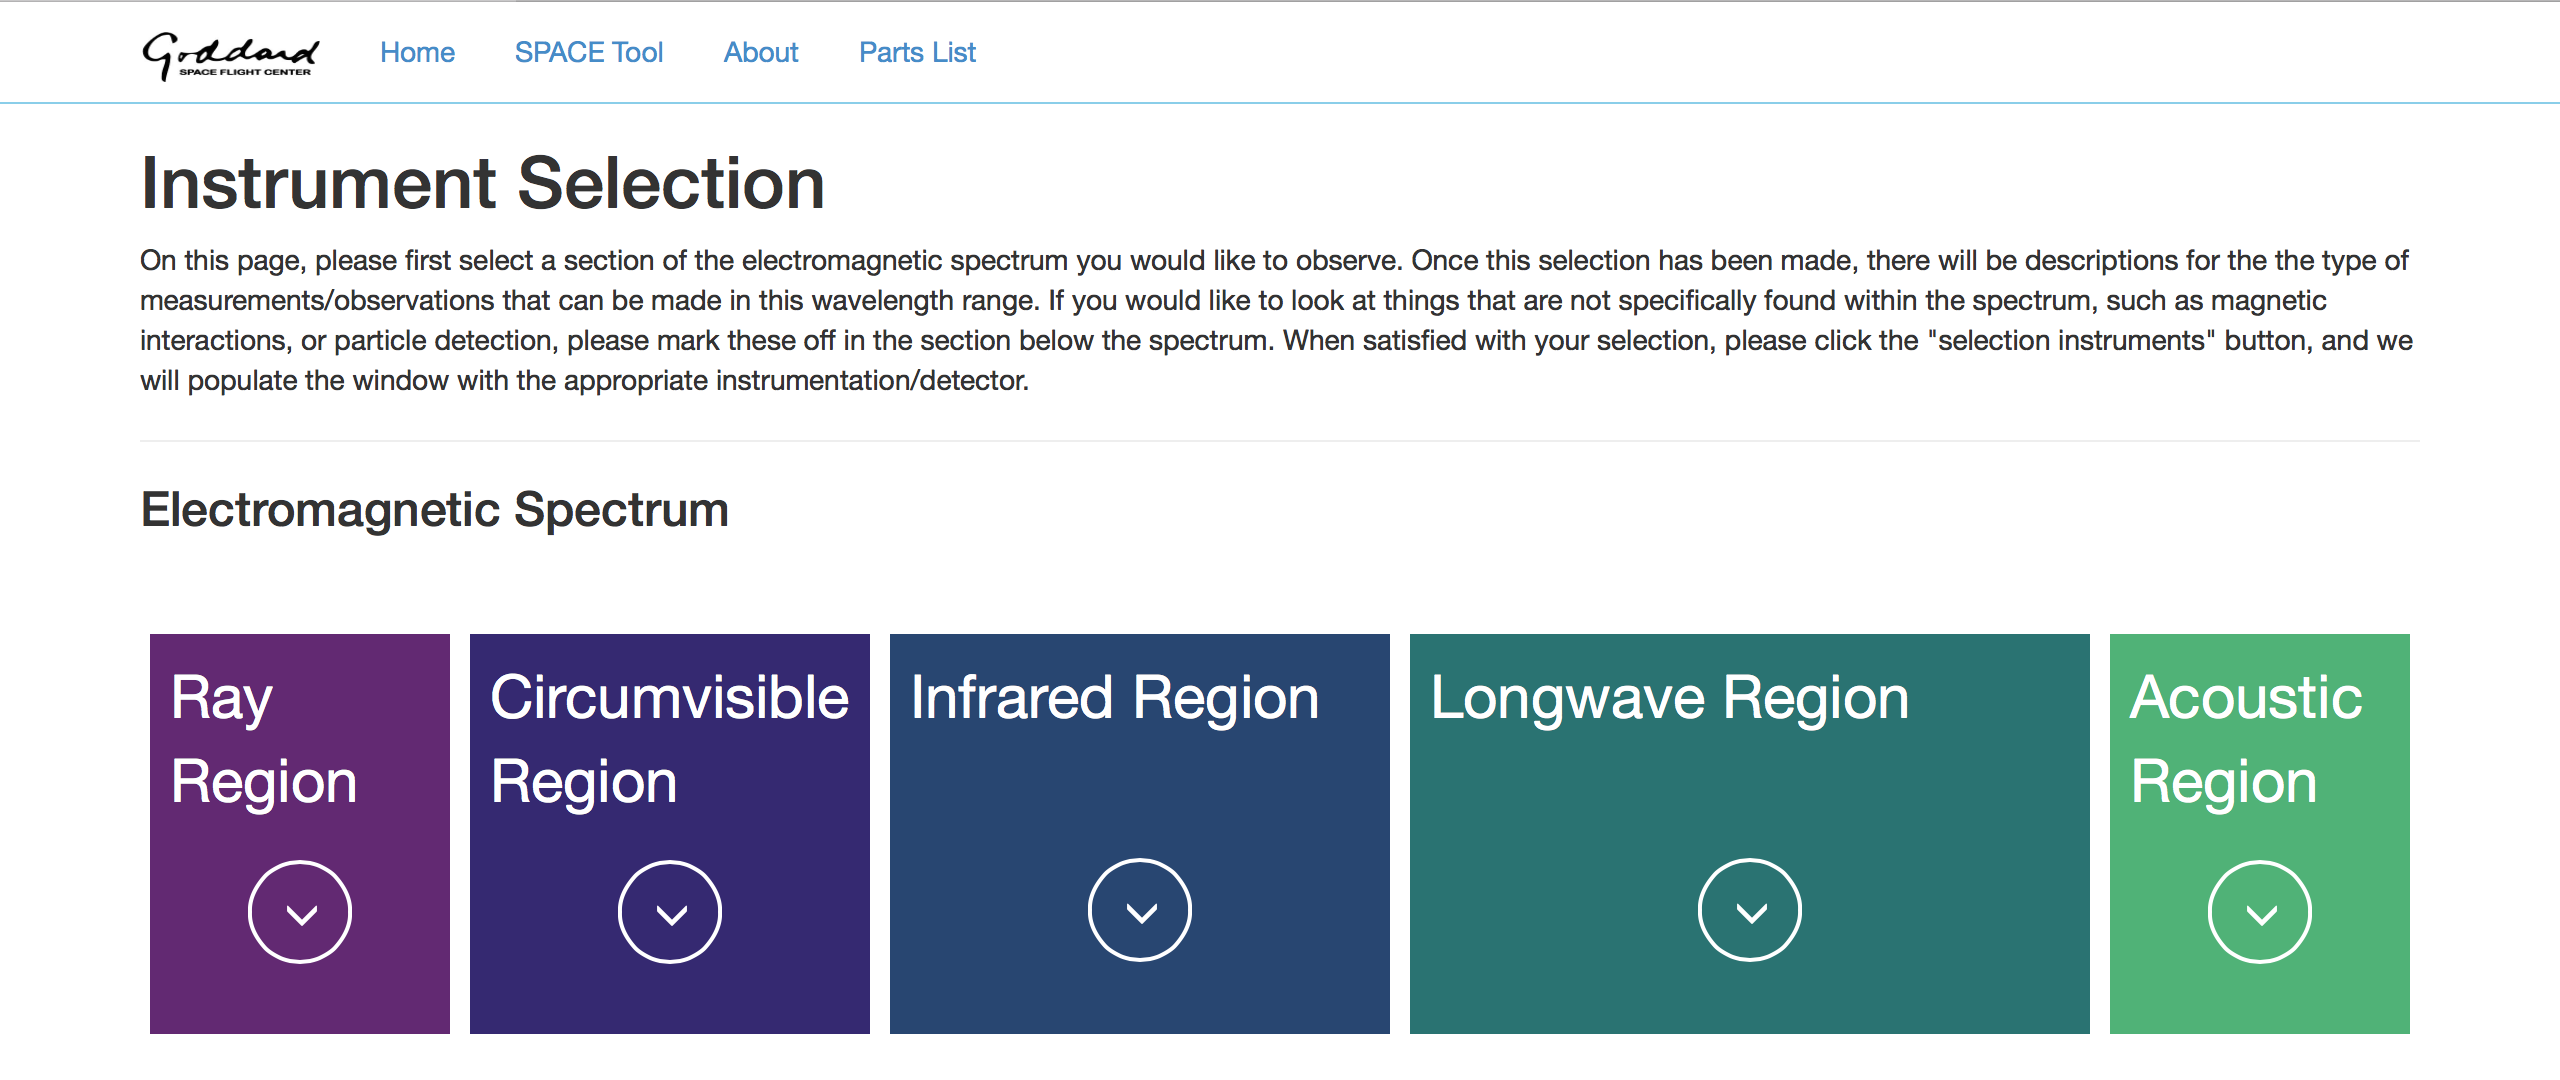
\includegraphics[width=\linewidth]{2a}
\caption{Screenshot of the Electromagnetic Spectrum}
\label{default}
\end{center}
\end{figure}

If the user wishes to bypass the electromagnetic spectrum approach, there is also an option for the user to mark off specifically what they would like to look at -- specifically with regards to fields, particles, and altimetry. These will effectively show all particle detectors, magnetometers, and altimeters to the user. However, the user interaction on this page will generally begin with a selection of a region of the spectrum based on the scale of the interactions they would like to observe, followed by the selection of a specific section of said region, which will show specifically the features they can measure. From there, the available instrumentation window will populate with the appropriate parts. The user can then read the description for each part, and choose what fits their mission best. 
\begin{figure}[H]
\begin{center}
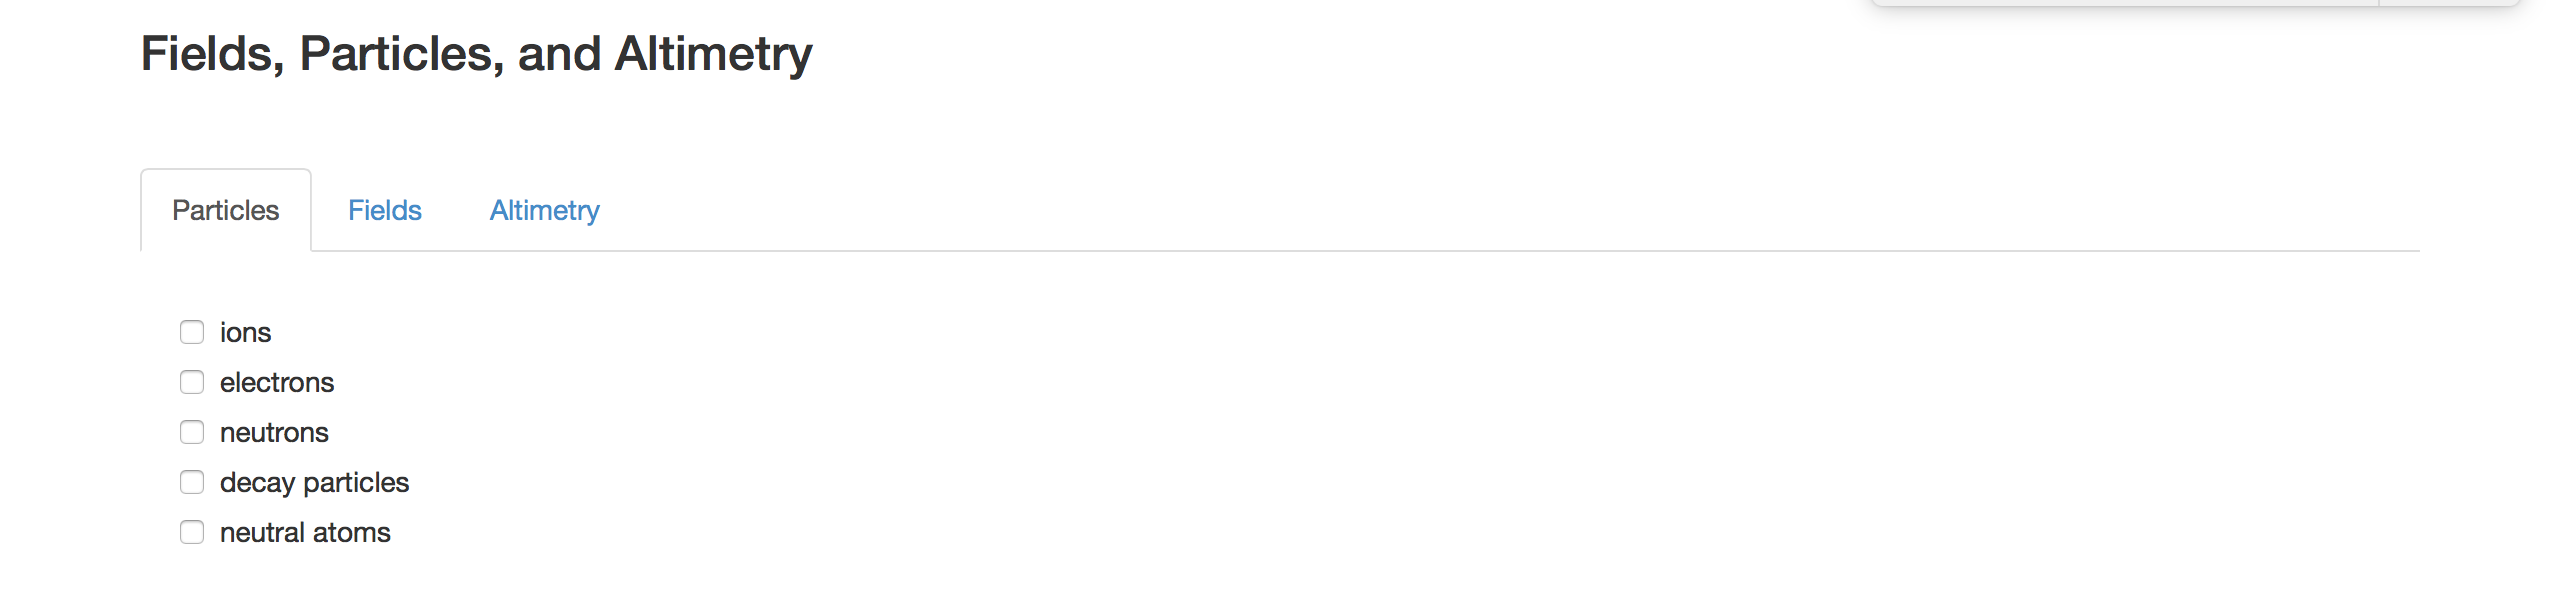
\includegraphics[width=\linewidth]{2b}
\caption{Screenshot of the instrumentation page (cont.)}
\label{default}
\end{center}
\end{figure}

\subsection{Attitude Control System Selection}
In this section, the user is asked to choose an attitude control system, sensors, or actuators, in order to perform attitude control for maneuvering as well as to maintain the resolution the user wishes to keep for their measurements. The algorithm asks for an altitude that your instrument will be stationed at, along with a maximum spatial resolution for your instrument. From these two fields, we will calculate an angle of knowledge, which will act as a driver for the angle of control (generally, the angle of knowledge needs to be 10 times better than the angle of control). The angle of knowledge is calculated as:
\begin{equation} \text{angle of knowledge} = \tan^{-1}\left(\dfrac{\text{spatial resolution}}{\text{altitude} * 1000}\right)\end{equation}
As mentioned, the angle of knowledge drives the angle of control:
\begin{equation} \text{angle of control} = \text{angle of knowledge} * 10 \end{equation}
We recommend that the user enters in something between 50-500km for their altitude, and 10-100m for their maximum spatial resolution. From there, we will display all subsystems that has an angle of precision lesser than or equal to the calculated angle of knowledge. We have within our database, ACS, sensors, as well as actuators, which the user can choose from. There is also an available option to sort the parts based on their mass, volume, or power. 
\begin{figure}[H]
\begin{center}
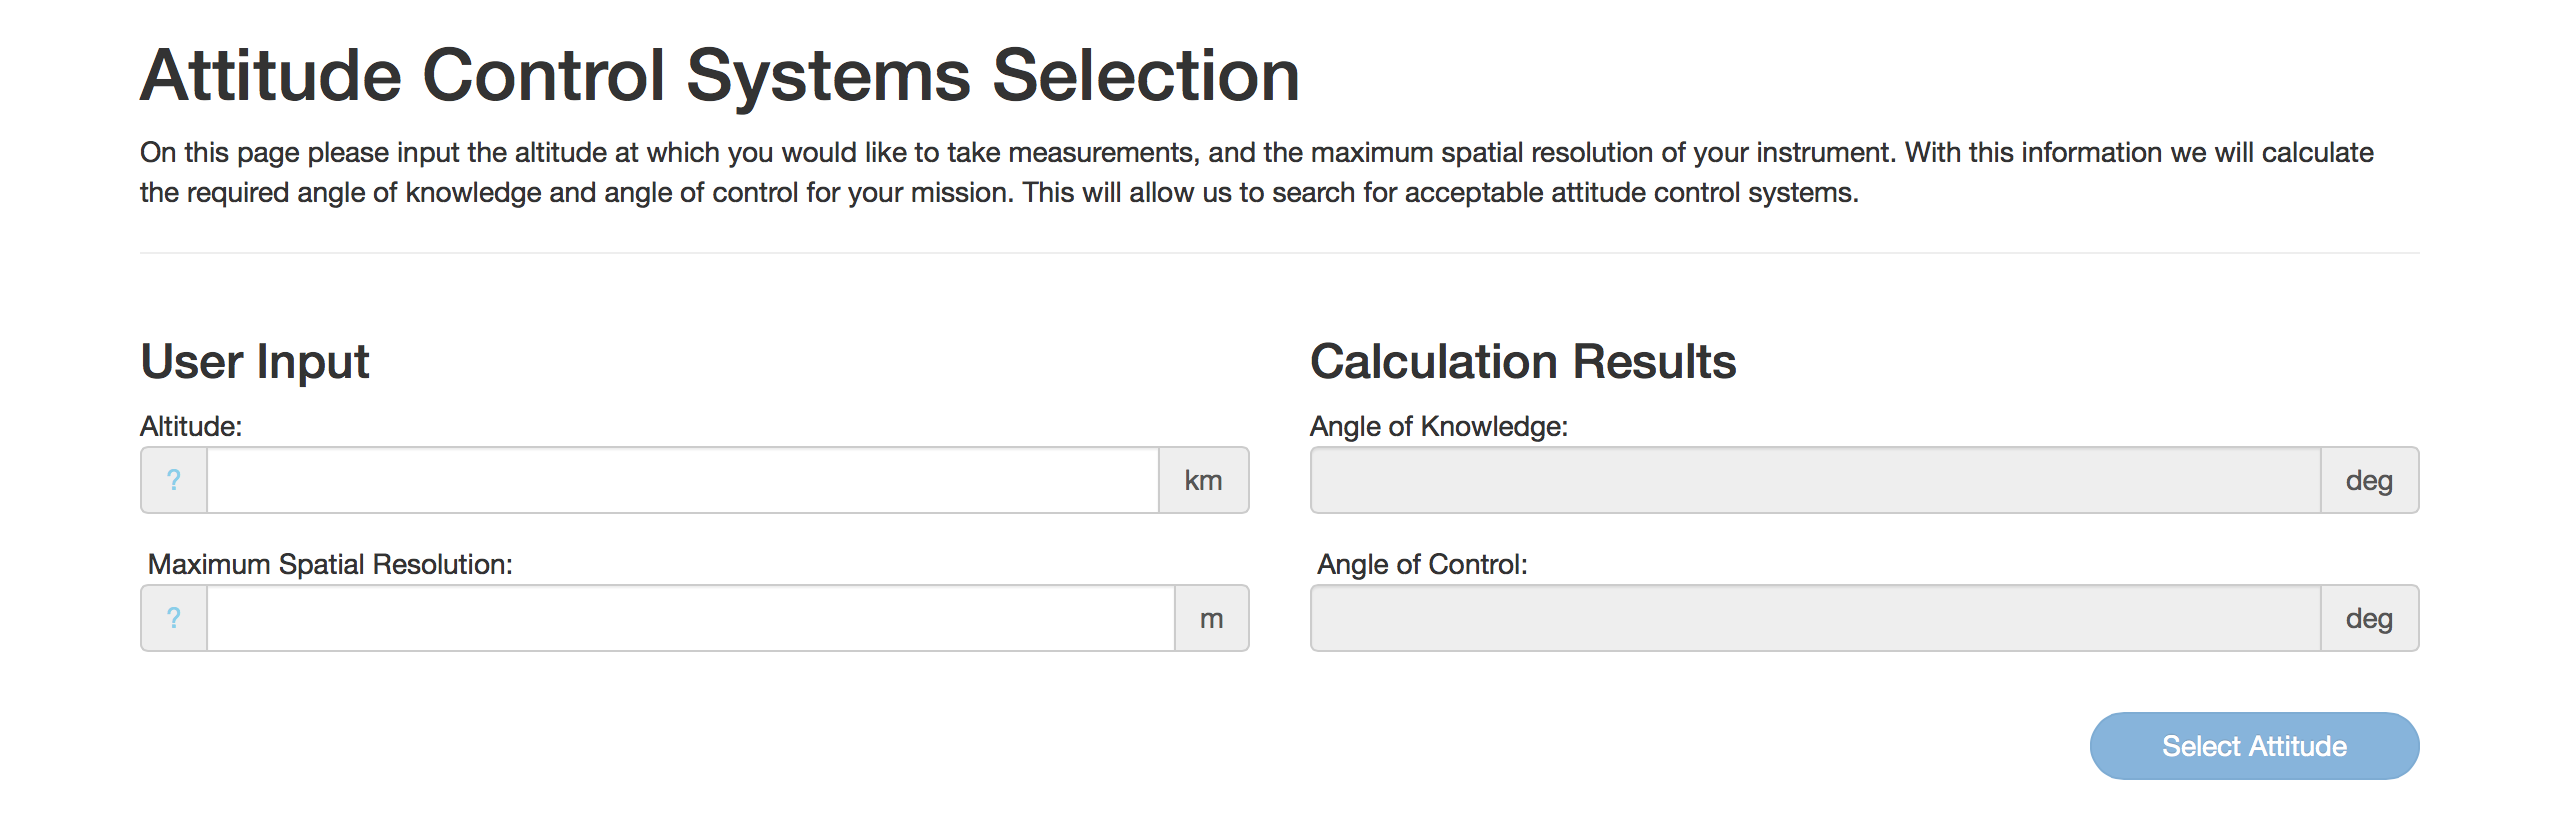
\includegraphics[width=\linewidth]{3}
\caption{Screenshot of the attitude control selection page}
\label{default}
\end{center}
\end{figure}

\subsection{Propulsion Selection}
In this section, the user will be able to calculate the total $\Delta$V required to get to the desired science orbit, which will be crucial in choosing the right propulsion system to provide the capabilities for navigation and maneuvering. It is important to have a capable propulsion system, especially when dealing with deep space CubeSats, as we can't just rely on passive navigation to get to the right orbit. For a more complicated trajectory, the total $\Delta$V can be calculated from a linear sum of individual $\Delta$V, also taking into account a change in inclination (if required). We have used some generalizations to generate the $\Delta$V for trajectories.\\[3mm] 
The user interaction has three separate parts, a direct/indirect $\Delta$V for getting to capture, a $\Delta$V for moving from capture to the science orbit, and an inclination change (if necessary). For the first stage, the page will ask the user whether they want a direct or indirect trajectory to the target of their choice -- from there, we will set this $\Delta$V internally. The user also has a choice to enter this value in manually. This value ranges from 0.01 to 3.0 km/s depending on the target. Next, the user is asked to enter an apoapsis and a periasis value for their science orbit. We have placed a table of suggested values for each body within this page, so the user has some guideline in the input values.
\begin{figure}[H]
\begin{center}
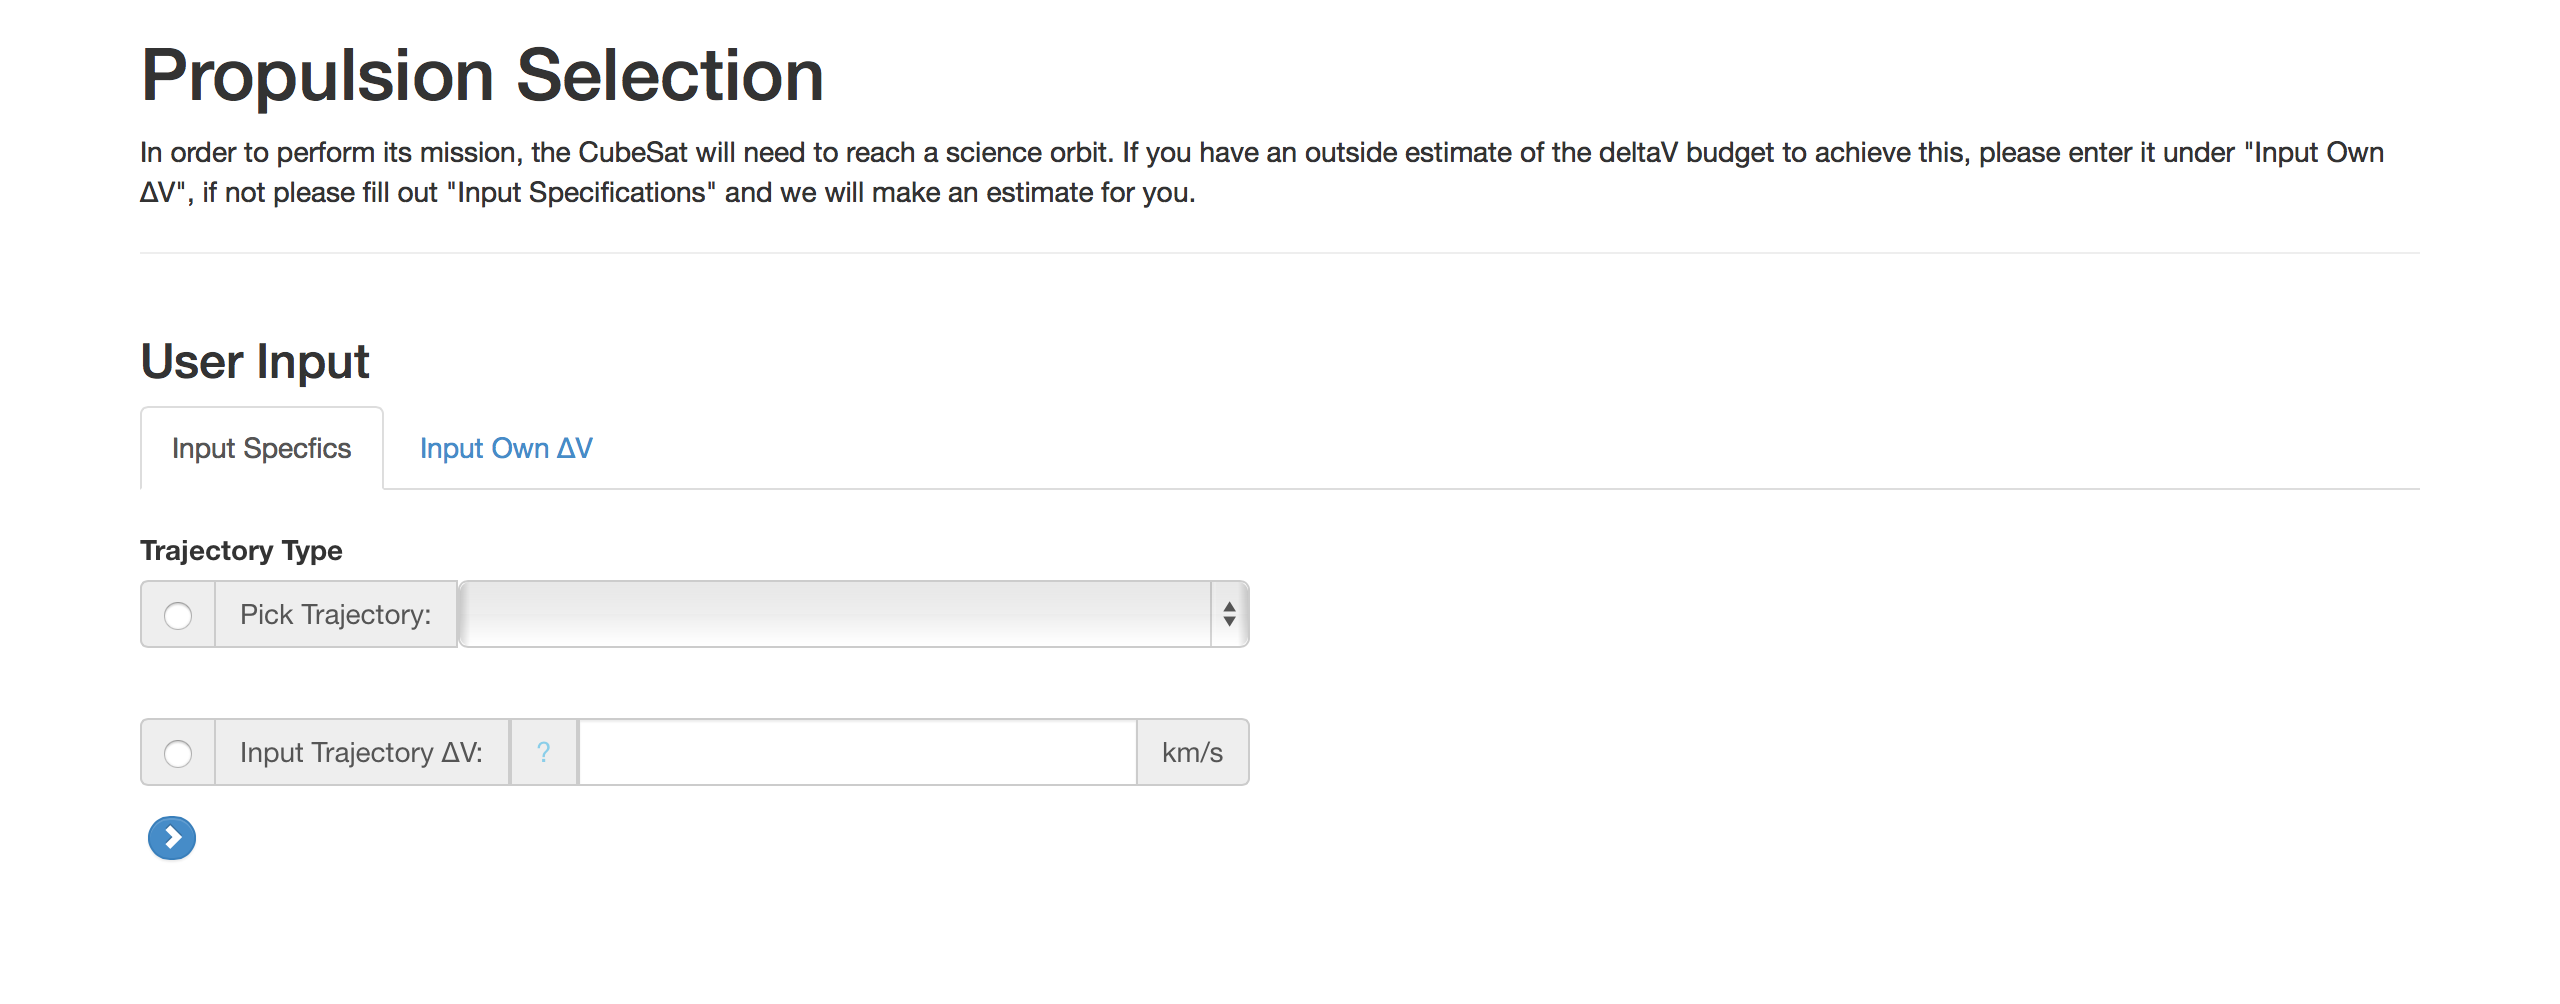
\includegraphics[width=\linewidth]{4a}
\caption{Screenshot of the trajectory selection page}
\label{default}
\end{center}
\end{figure}

\begin{figure}[H]
\begin{center}
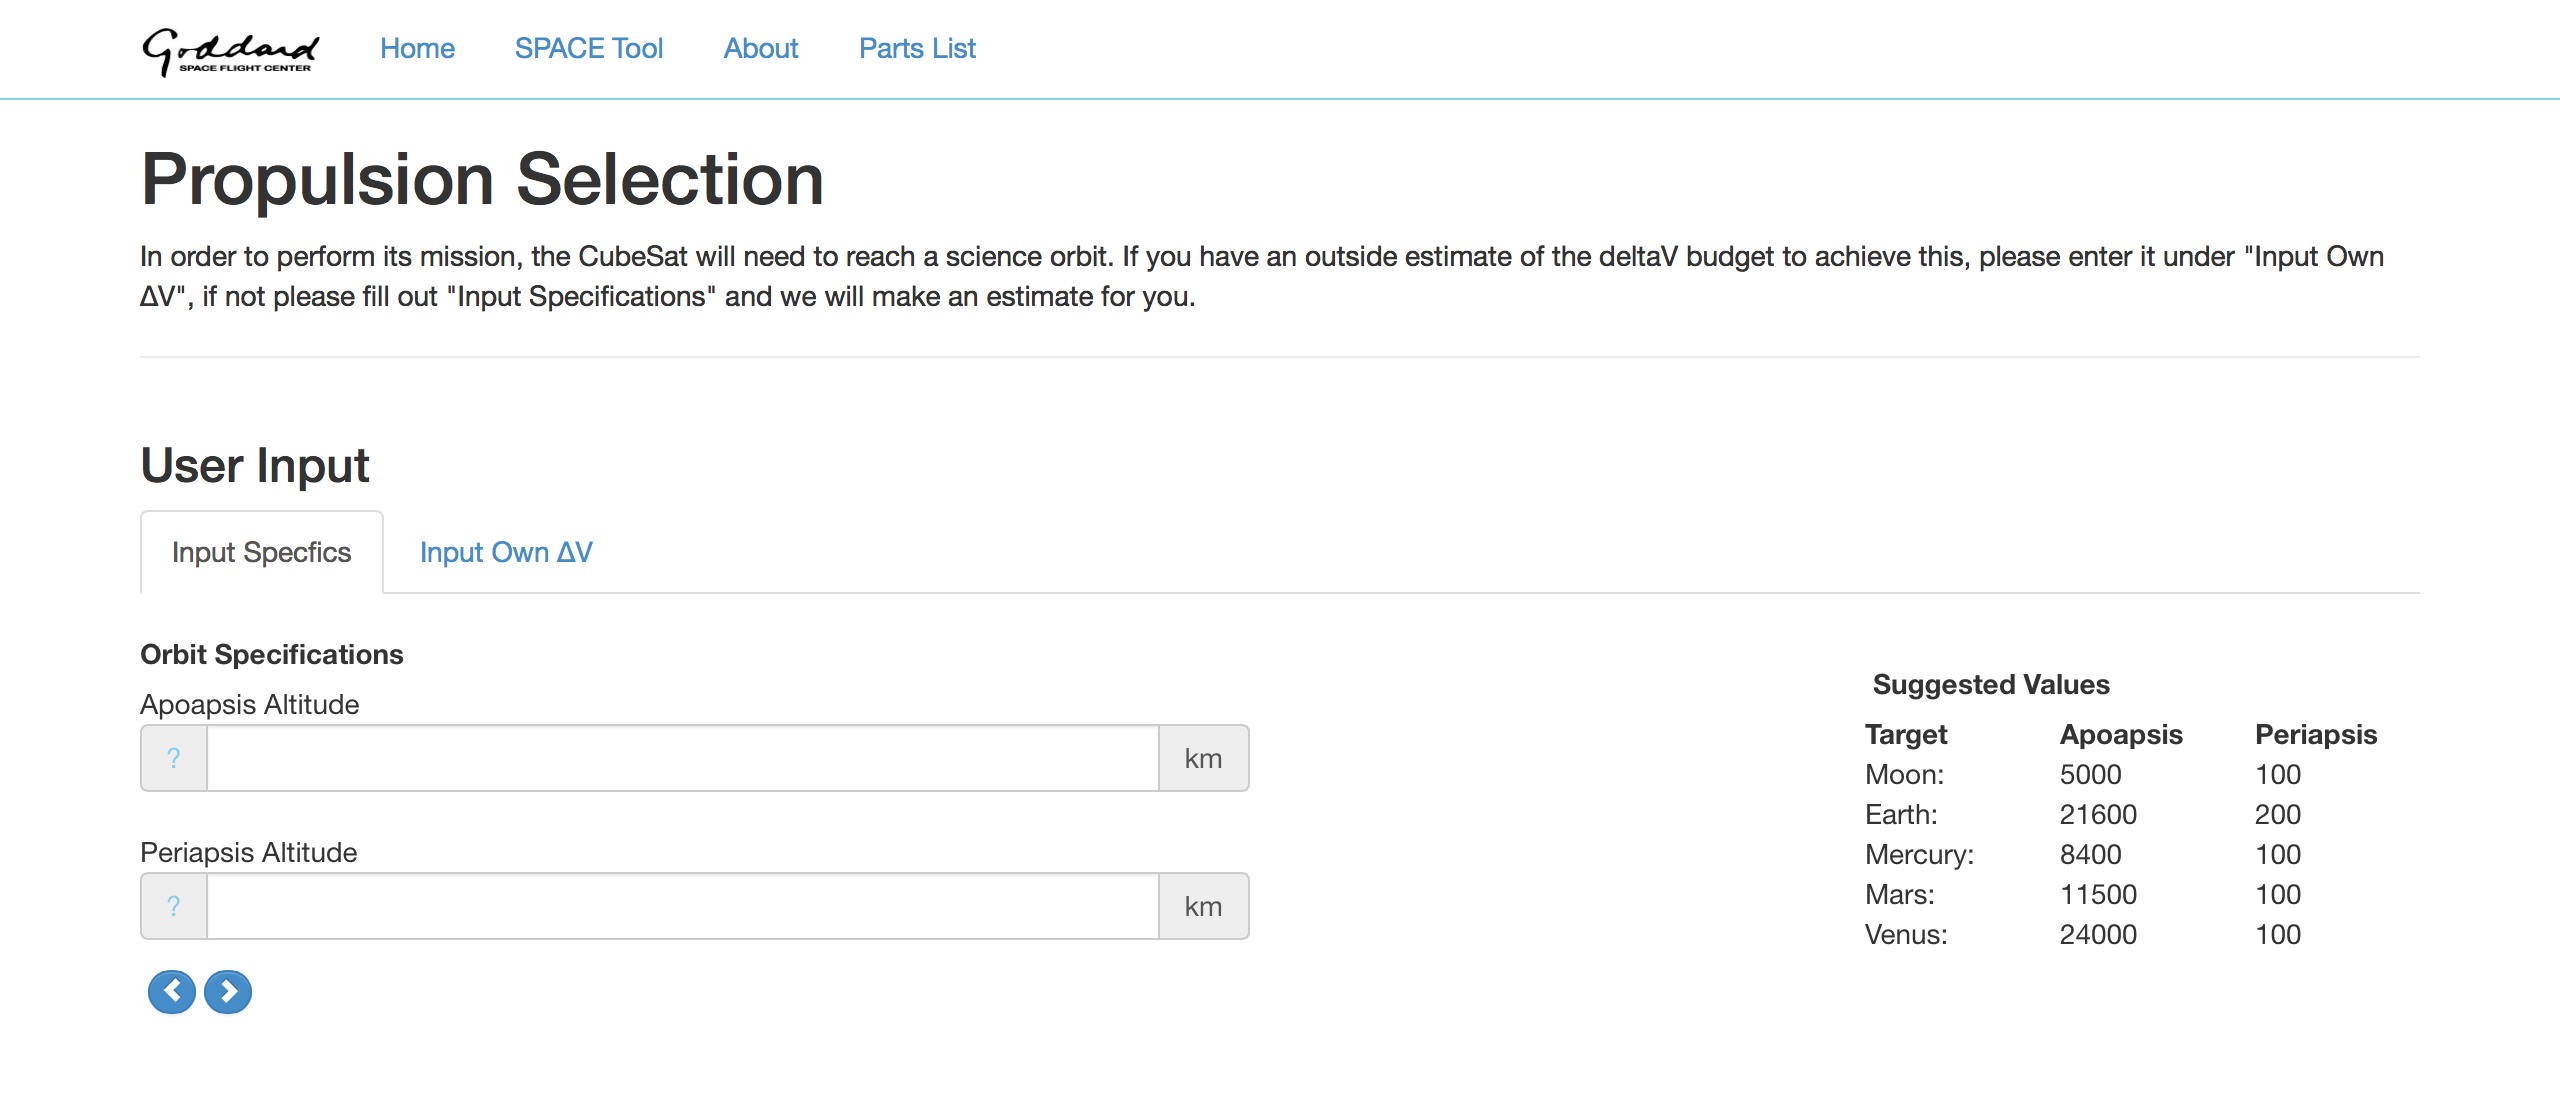
\includegraphics[width=\linewidth]{4b}
\caption{Screenshot of the trajectory selection page (cont.)}
\label{default}
\end{center}
\end{figure}

\begin{figure}[H]
\begin{center}
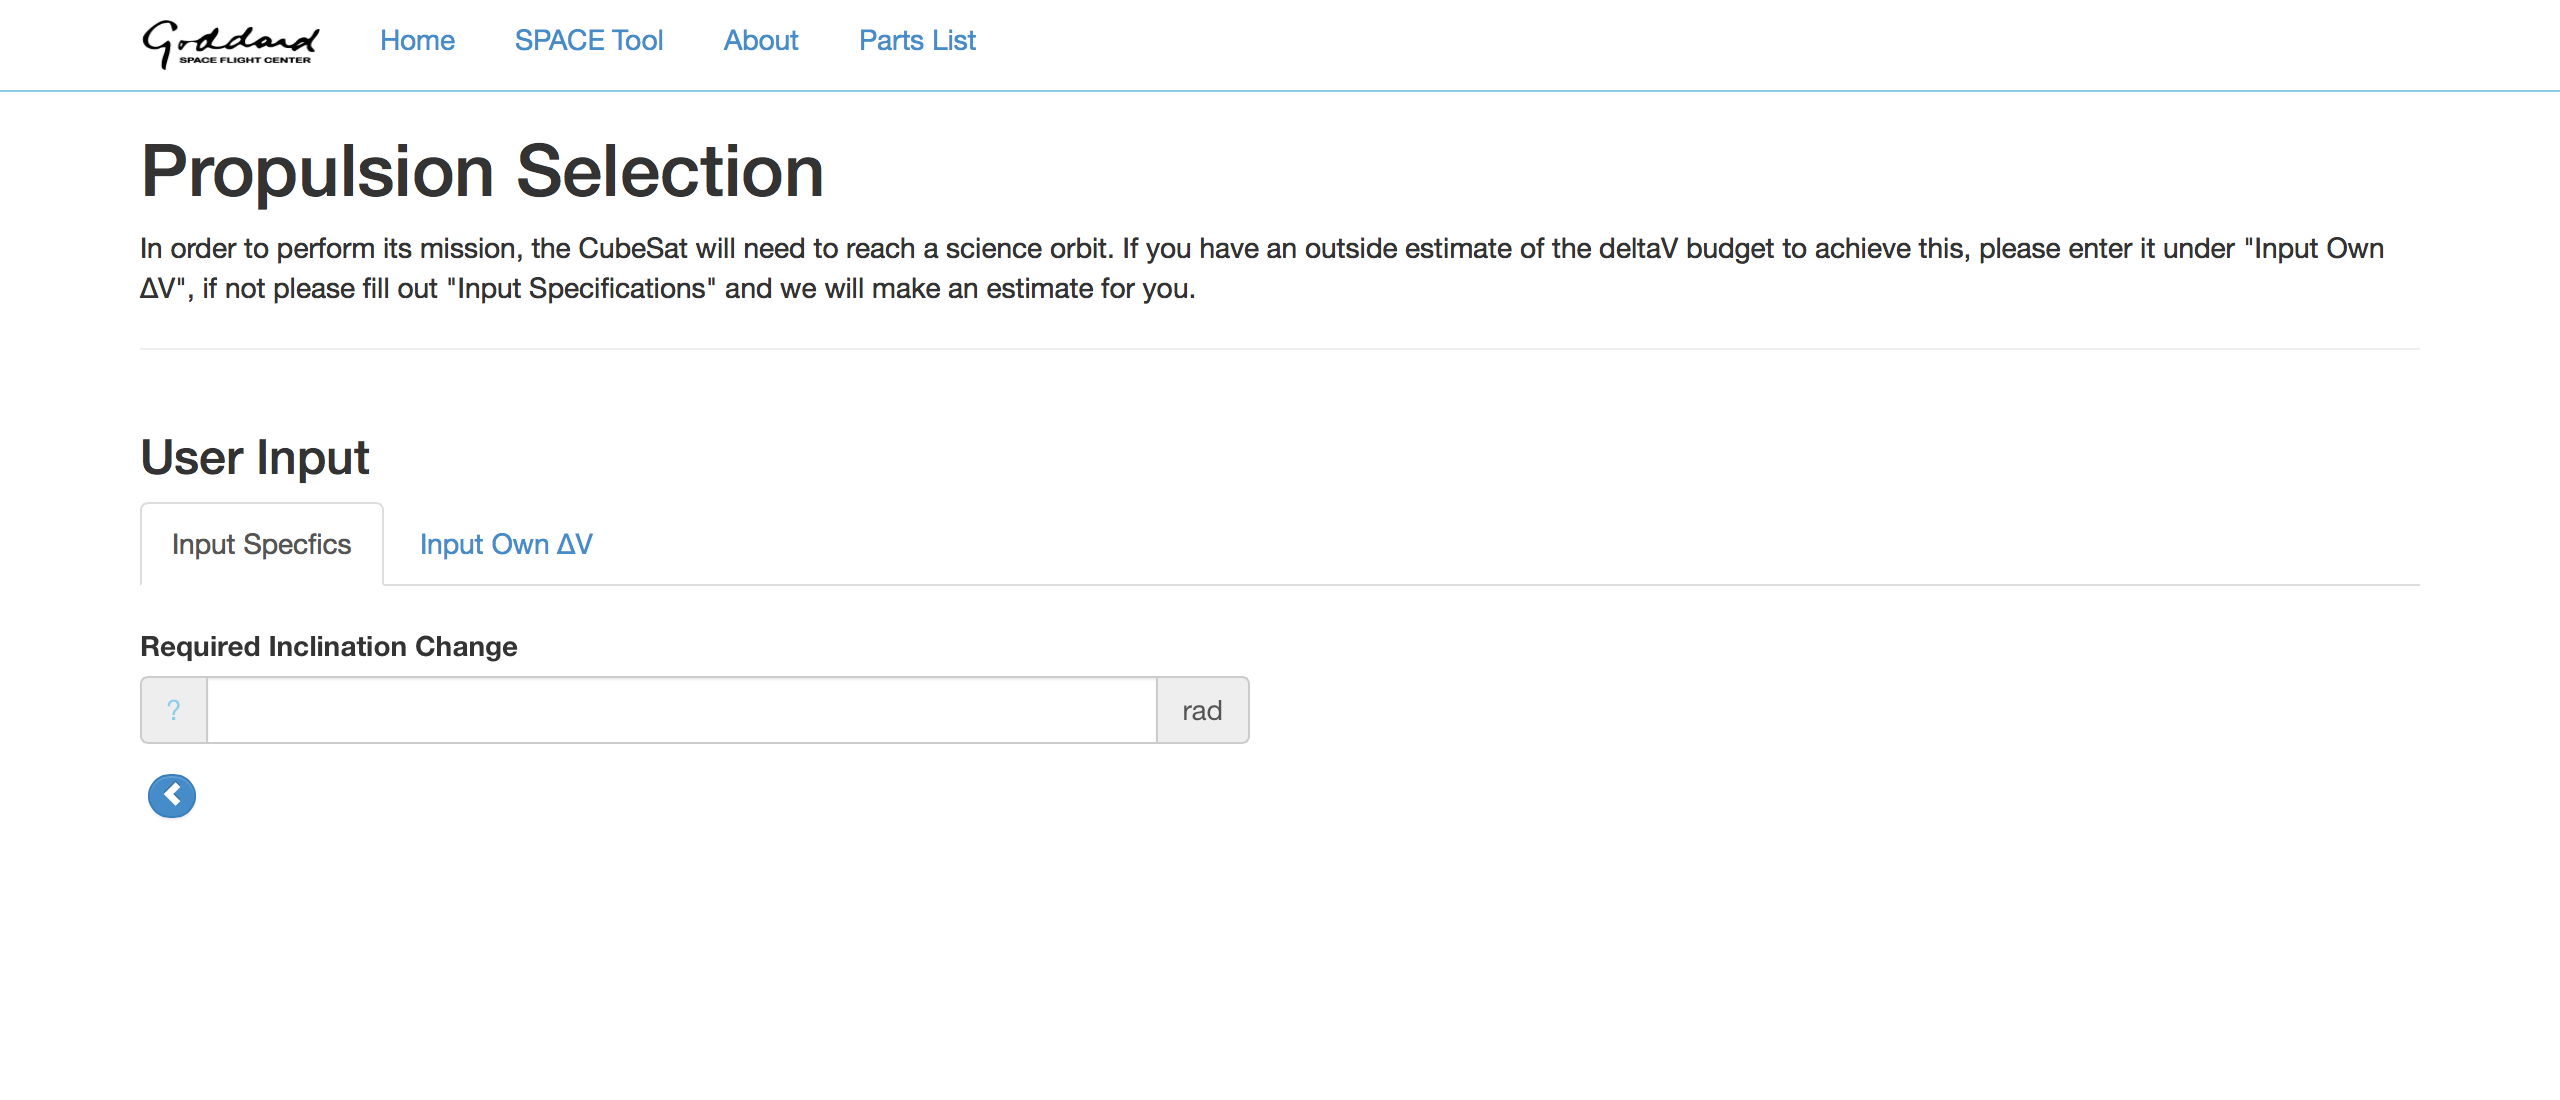
\includegraphics[width=\linewidth]{4c}
\caption{Screenshot of the trajectory selection page (cont.)}
\label{default}
\end{center}
\end{figure}

\noindent Finally, the user is asked for an inclination change, which they may put in zero if not required. We have put the values of the suggested apoapsis/periapsis values below:
\begin{table}[H]
\caption{Suggested apoapsis/periapsis values}
\begin{center}
\begin{tabular}{|c|c|c|}
\hline
Body & Apoapsis (km)& Periapsis (km) \\
\hline
Moon & 5000 & 100 \\
Earth & 21600 & 200\\
Mercury & 8400 & 100\\
Mars & 11500 & 100\\
Venus & 24000 & 100\\
\hline
\end{tabular}
\end{center}
\label{default}
\end{table}%
%
%\begin{table}[H]
%\caption{$\Delta$V for getting into capture}
%\begin{center}
%\begin{tabular}{|c|c|c|}
%\hline
%Body & Type & $\Delta$V (km/s)\\
%\hline
%Earth - low & Direct & \\
%& Indirect & \\
%\hline
%Earth - medium & Direct & \\
%& Indirect & \\
%\hline
%Earth - high & Direct & \\
%& Indirect & \\
%\hline
%Moon & Direct & \\
%& Indirect & \\
%\hline
%Mercury & Direct & \\
%& Indirect & \\
%\hline
%Mars & Direct & \\
%& Indirect & \\
%\hline
%Venus & Direct & \\
%& Indirect & \\
%\hline
%\end{tabular}
%\end{center}
%\label{default}
%\end{table}
\noindent Once the final value has been calculated, we can filter down and find the appropriate propulsion mechanisms according to the $\Delta$V budget. Note that there is also a form to fill in the $\Delta$V beforehand, if the user knows what it is. The user can also choose to filter further and choose from thrusters or sails, and sort by mass, power, or volume.\\[3mm]
Currently, we are trying to work out some bugs within the apoapsis/periapsis calculations. If the user enters in the suggested values, they will get a reasonable $\Delta$V (under 5 km/s). However, if they begin straying away from these values (namely $\pm$5 km), the $\Delta$V will blow up into the hundreds of thousands of km/s. We have sought advice from an orbital mechanics expert, and are continuing to work on this issues. 
\subsection{Communication Selection}
In this section, the user will be guided in choosing an antenna, receiver, and ground station from a selected band in order to perform the communication from orbit to ground station. We currently have parts for the VHF, UVF, S, and X band, which ranges from .3 GHz to 12 GHz. More specifically:
\begin{enumerate}
\item VHF (Very High Frequency): ranges from 30 MHz to 300 MHz. Its common uses are FM radio broadcasting, television broadcasting, two way land mobile radio systems, long range data communication up to several tens of kilometers.
\item UHF (Ultra High Frequency): ranges from 300 MHz to 3 GHz. Its common uses are television broadcasting, cell phones, satellite communication including GPS, personal radio services including wifi and Bluetooth, walkie-talkies, cordless phones, and numerous other applications.
\item S-band: ranges from 2 GHz to 4 GHz. Its common uses are weather radars, surface ship radars, some communications satellites, especially those used by NASA to communicate with the Space Shuttle and the International Space Station.
\item X-band: ranges from 4 GHz to 12 GHz. Portions of the X band are assigned by the International Telecommunications Union (ITU) exclusively for deep space telecommunications. The primary user of this allocation is the American NASA Deep Space Network (DSN) which is a network of large dish antennas located all over the world to provide overlapping global coverage.
\end{enumerate}
\begin{figure}[H]
\begin{center}
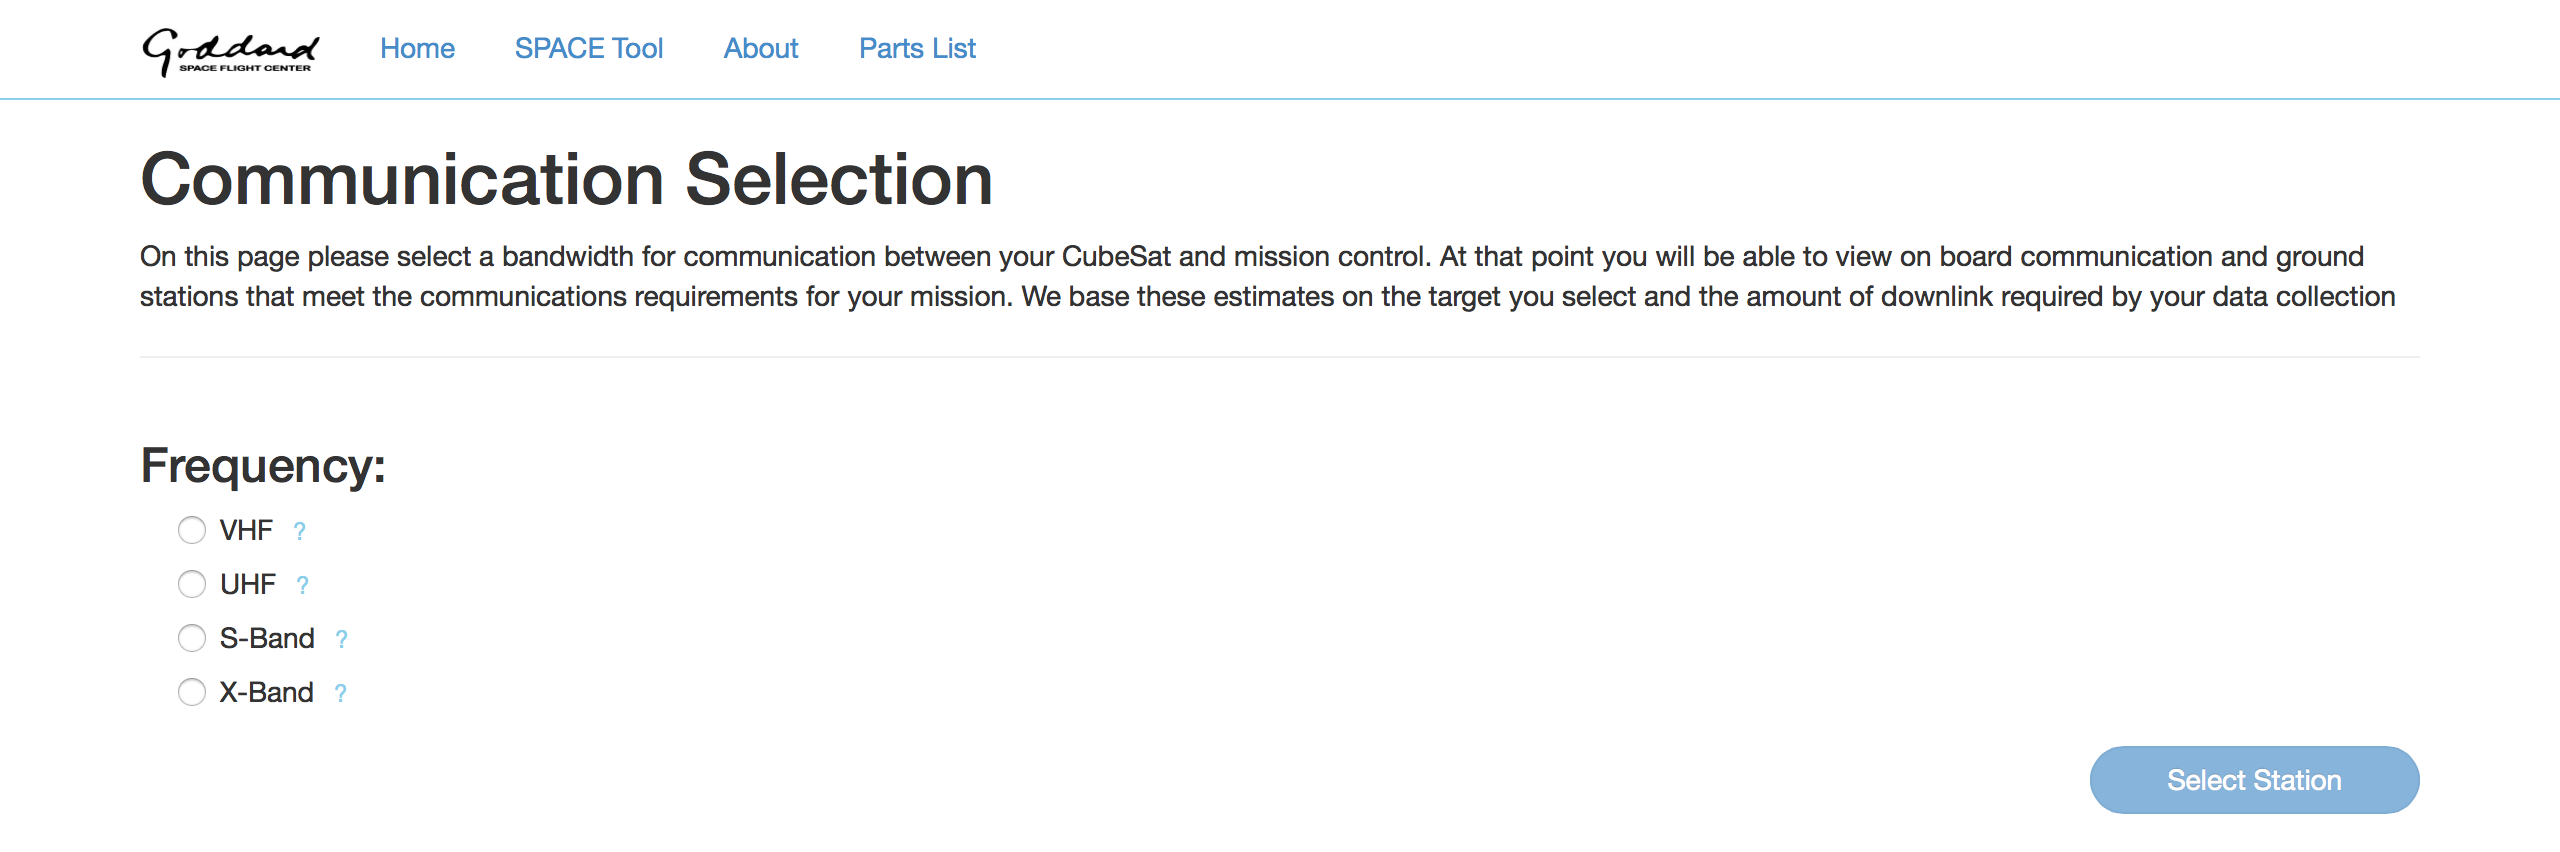
\includegraphics[width=\linewidth]{5}
\caption{Screenshot of the communication selection page}
\label{default}
\end{center}
\end{figure}
Because of its limitations in available mass and power, spacecraft have relatively low power transmitter/receiver systems. We can bypass this by using  small dish antennas on the CubeSats, which will focus the signal into a narrow beam in order to minimize space loss. On the receiving side, the signal can be amplified with large dish signals, and further processed to remove most noise. The transmitting signal has also been modulated in order to send the signal over a bandpass frequency range with a carrier signal.\\[3mm]
Once the antenna, receiver, and ground station are chosen for an associated band, we will calculate a free-path space loss term, a receive power term, a signal to noise ratio, and a maximum bit rate achievable by the chosen subsystem using known values of the chosen parts. The free-path space loss term (dB) is calculated as:
\begin{equation} \text{space loss} = 20*\log_{10}\left(\dfrac{4*\pi*\text{dist}*\text{frequency}}{c}\right)\end{equation}
where c = speed of light (3$\times$10$^8$), frequency = transmitted frequency, distance = distance from transmitter to receiver. We'll include here a table of and distances frequencies used in our calculation:
\begin{table}[H]
\caption{Distances from Earth to specified target}
\begin{center}
\begin{tabular}{|c|c|}
\hline
Target & Distance (m)\\
\hline
Earth - low & 2,000,000\\
Earth - medium & 2,020,000\\
Earth - high & 4,000,000 \\
Moon & 384,400,000\\
Mercury &  2.22$\times10^{11}$\\
Venus & 2.61$\times10^{11}$\\
Mars & 4.01$\times10^{11}$\\
\hline
\end{tabular}
\end{center}
\label{default}
\end{table}%
\begin{table}[H]
\caption{Frequencies associated with each band}
\begin{center}
\begin{tabular}{|c|c|}
\hline
Band & Frequency (Hz)\\
\hline
VHF & 0.165$\times10^{9}$\\
UHF & 1.65$\times10^{9}$\\
S & 3$\times10^{9}$\\
X & 8.49$\times10^{9}$\\
\hline
\end{tabular}
\end{center}
\label{default}
\end{table}%
The receive power term (dBW) is calculated as:
\begin{equation} \begin{aligned} \text{receive power} = & \text{ transmitter output power} + \text{transmit antenna gain} \\ &- \text{cable losses} - \text{space loss} + \text{antenna gain} \end{aligned} \end{equation}
For transmitter output power, we are using a standard figure of approximately 20 dBW, For antenna cable loss, we are using another standard figure of approximately 1 dB. For transmit antenna gain, it is calculated as:
\begin{equation} 20 * \log_{10} \left(\dfrac{\pi d}{ \lambda}\right) \end{equation}
where $\lambda=c / \text{frequency}$ and $d$ is the parabolic dish diameter (typically 0.5 meters). The space loss was calculated in formula (3). The antenna gain is a value attached to the antenna part chosen. The signal to noise ratio (dB) is calculated as:
\begin{equation} \text{SNR} = \text{receive power} - (10 * \log_{10}(kTB))\end{equation}
where receive power was calculated in formula (4). k is Boltzman's constant ($1.3807\times10^{-23}$), T is the temperature of the Earth (290K), and B is the bandwidth (1 MHz). The maximum bit rate (Kbps) is calculated using Shannon's theorem:
\begin{equation} \text{bit rate} = B_{\text{transmit}} * \log_2\left(1 + \left(10^{(SNR - 33.3) / 10)}\right)\right) / 1000 \end{equation}
We are fairly confident in the results of the other three terms we have calculated in this page, however, we had to take some generalities in the bit rate formula in order to get a figure that is on the scale of reasonable. First, in order to modify the SNR (signal to noise ratio), we have to subtract 30 dB for carrier detection, then an addition 3.3 dB for a link margin. Depending on the parts and band chosen, this usually leaves us with a figure of about 10 dB, which if we were using a binary phase shift keying (BPSK) modulation scheme, would be enough to get a bit error rate (BER) of 1E-6 for no or trivial dynamics. We also used a transmitted bandwidth of 1 kilohertz in this formula, but realistically, this value would be modified depending on the mission and what's required in terms of downlink rate.\\[3mm] 
In consulting with an industry expert, we found that the bit rate is usually set as a free variable (depending on mission requirements) and engineers will figure out what's needed to get to get to that bit rate. In our algorithm, we have presented a rough formula for finding the maximum bit rate that your system is capable of. However, we have taken many generalities in order to get to that number. With future iterations to this software, we hope to come up with a more quantifiable approach in our calculation. 
\subsection{Command and Data Handling Selection}
In this section, the user will be able to find an appropriate command and data handling subsystem capable of receiving, transmitting, processing and storing the data generated during the mission. First, the algorithm will ask you to fill in some information about the collection system in order to find the minimum number of kilobits generated per second during the process of acquiring data. There are three ways the user can enter in this data:
\begin{enumerate}
\item Number of channels $\times$ bits per channel $\times$ integration interval per second. 
\item Array size (x) $\times$ array size (y) $\times$ integration interval per second.
\item Bits per second (if they know the number firsthand)
\end{enumerate}
\begin{figure}[H]
\begin{center}
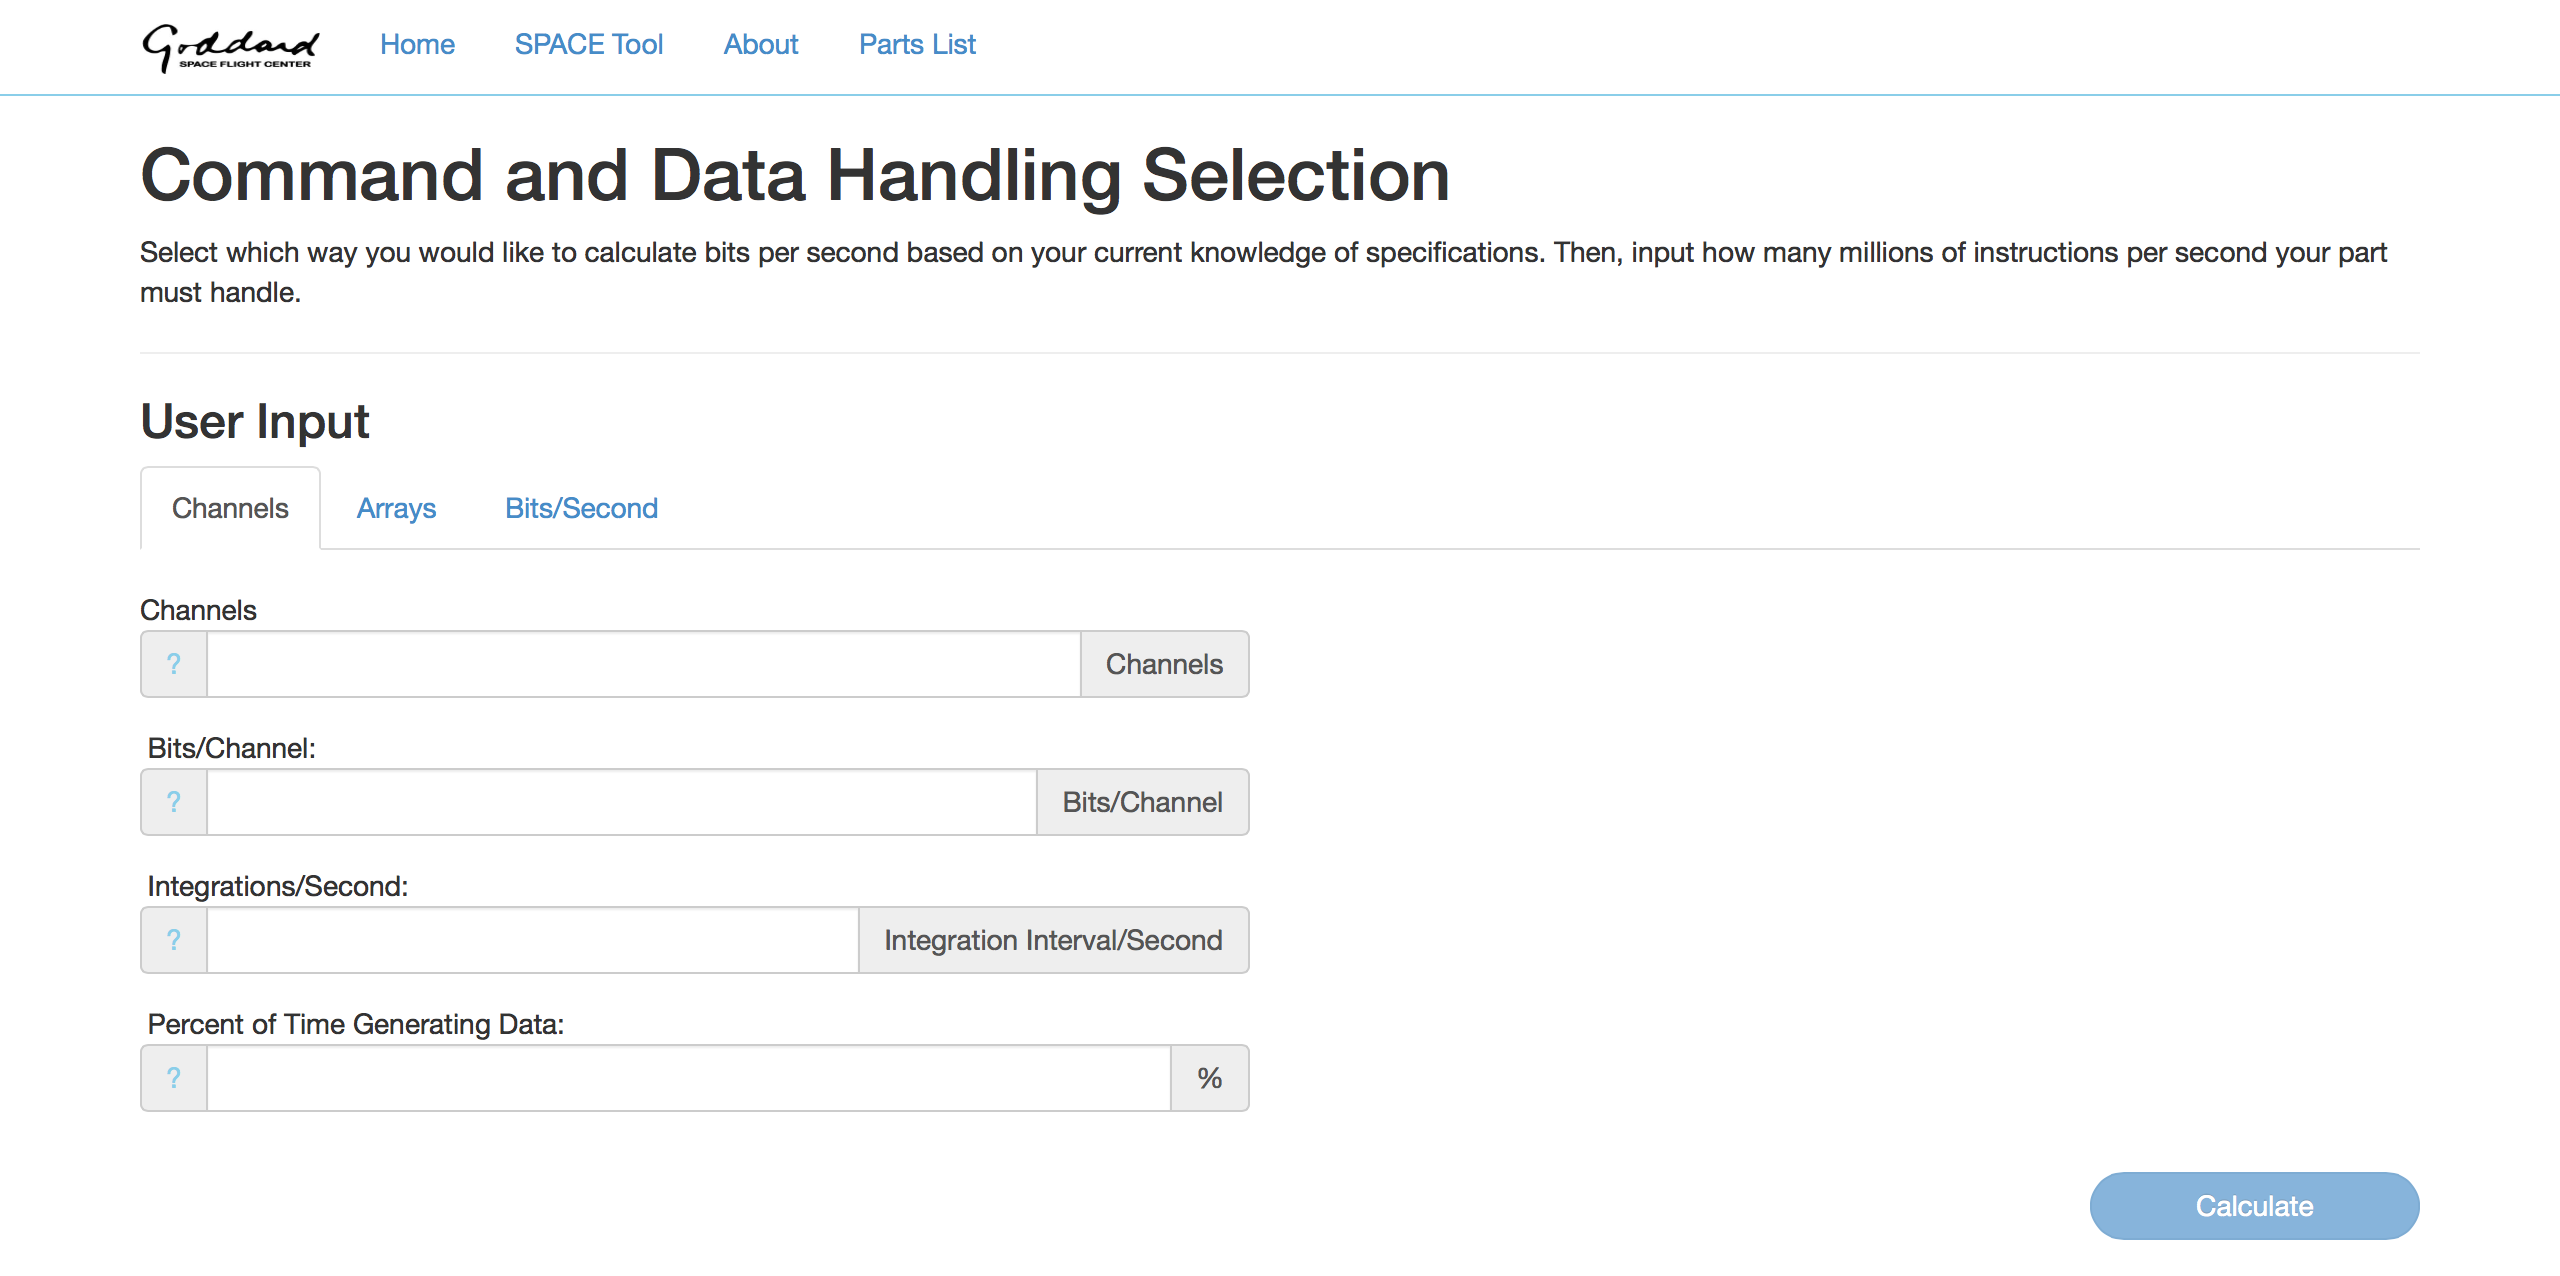
\includegraphics[width=\linewidth]{6a}
\caption{Screenshot of the CDH selection page (cont.)}
\label{default}
\end{center}
\end{figure}
\begin{figure}[H]
\begin{center}
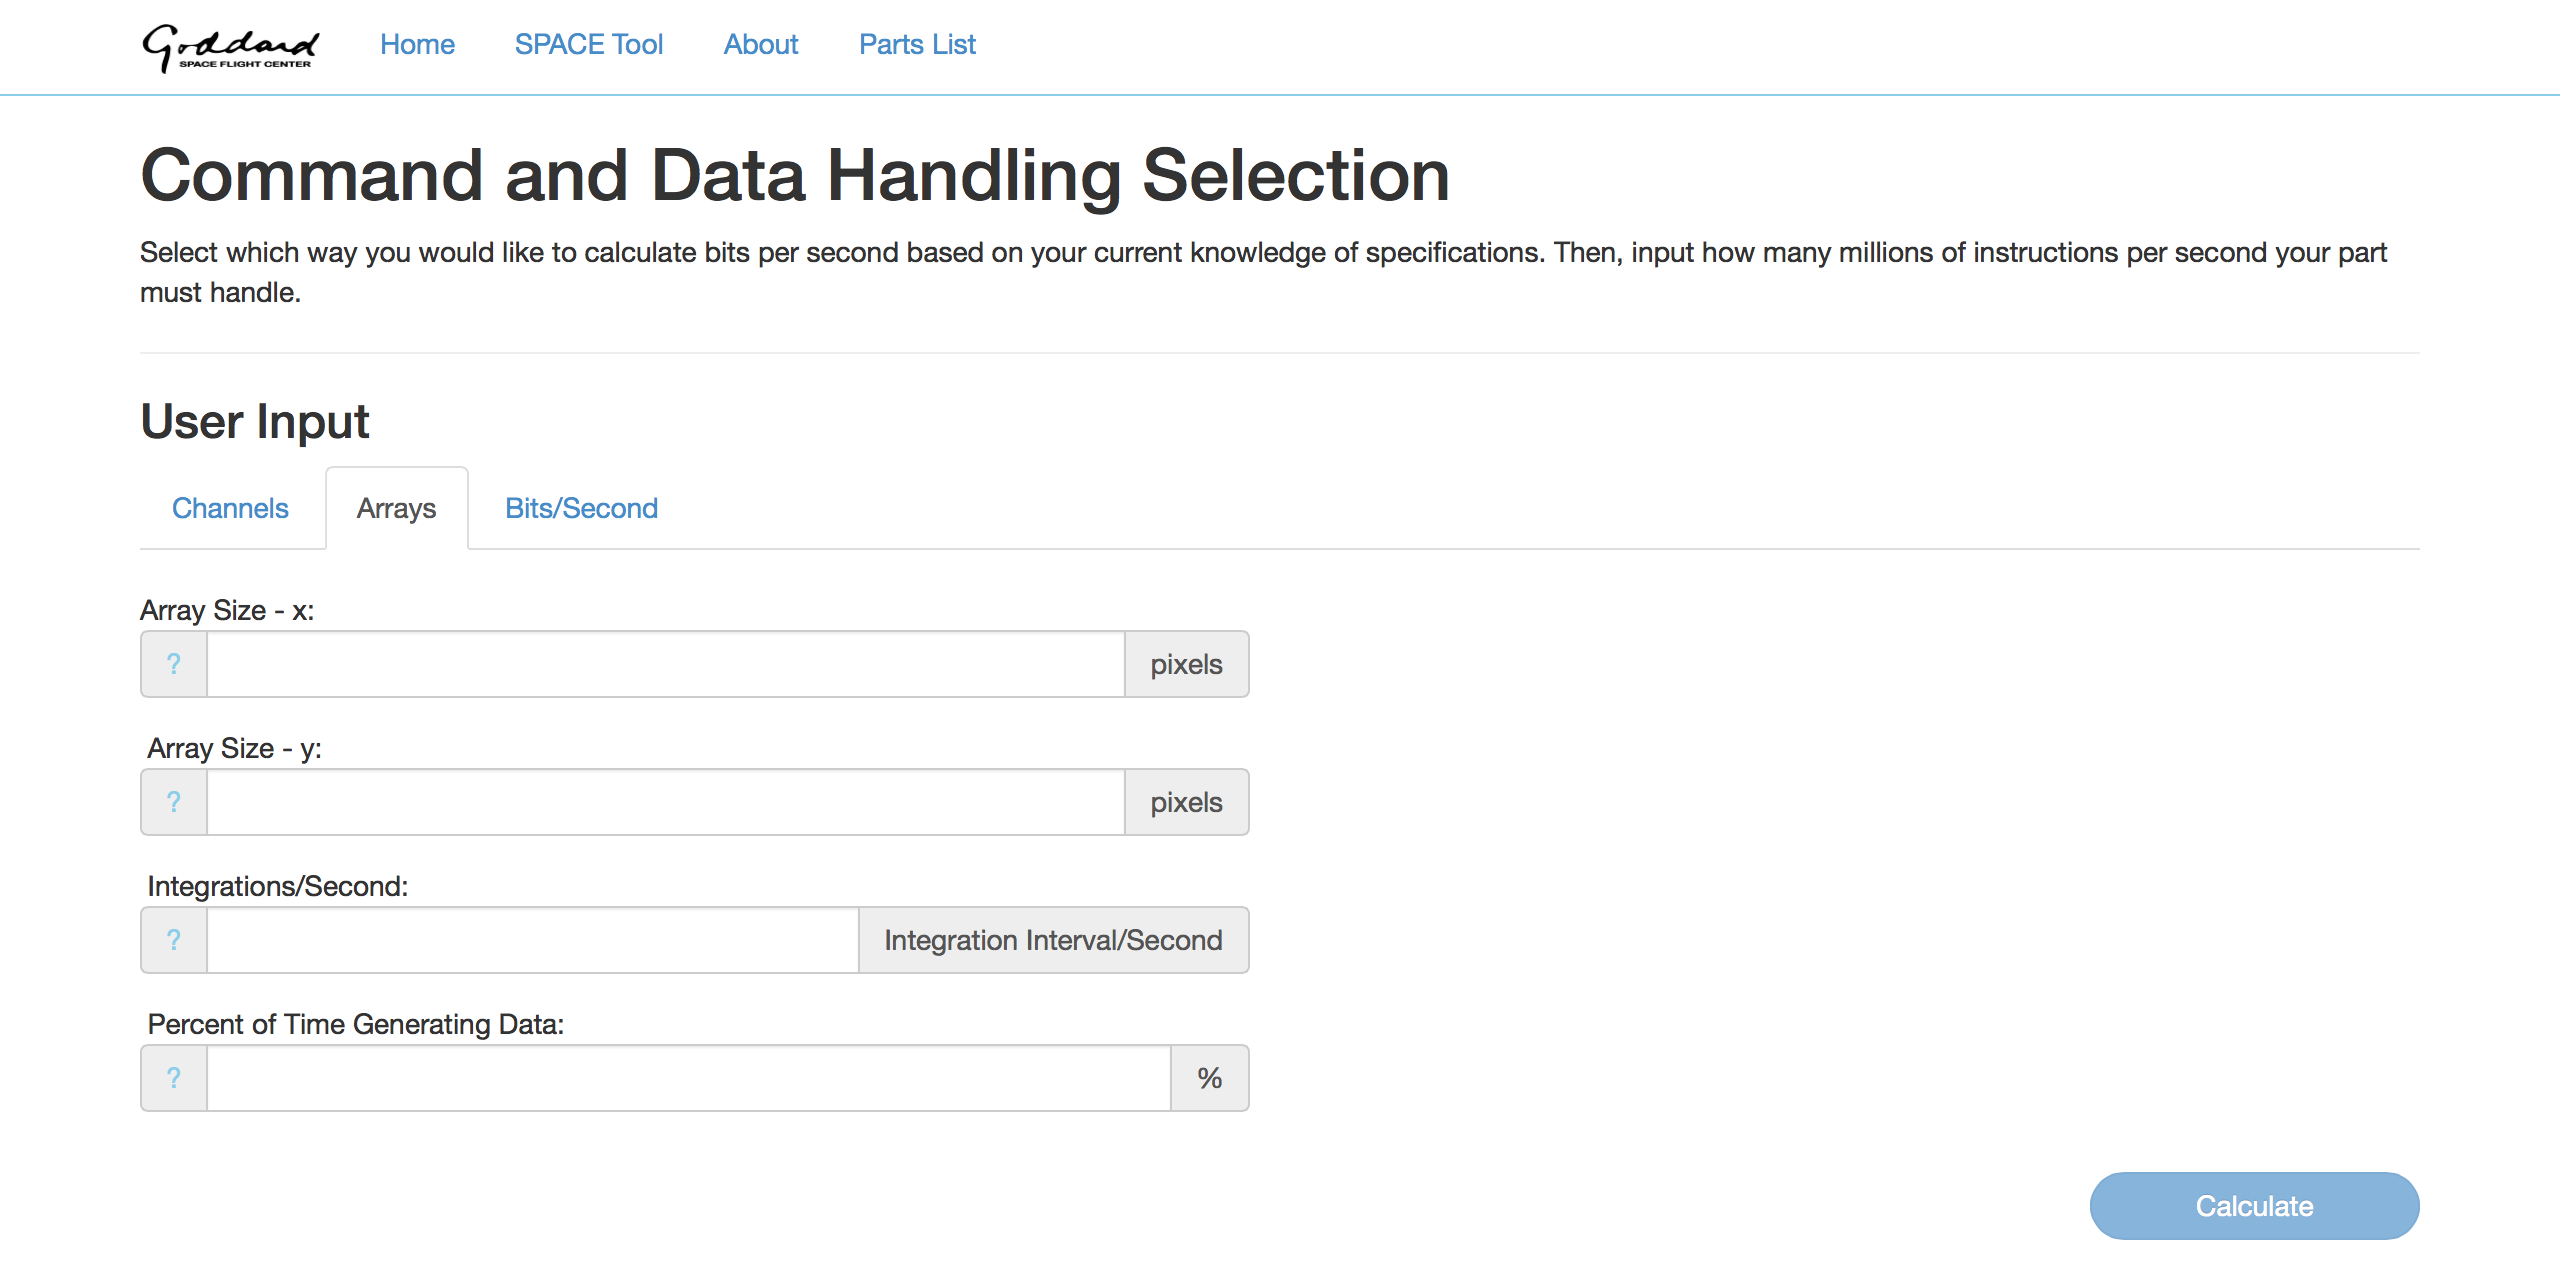
\includegraphics[width=\linewidth]{6b}
\caption{Screenshot of the CDH selection page (cont.)}
\label{default}
\end{center}
\end{figure}\begin{figure}[H]
\begin{center}
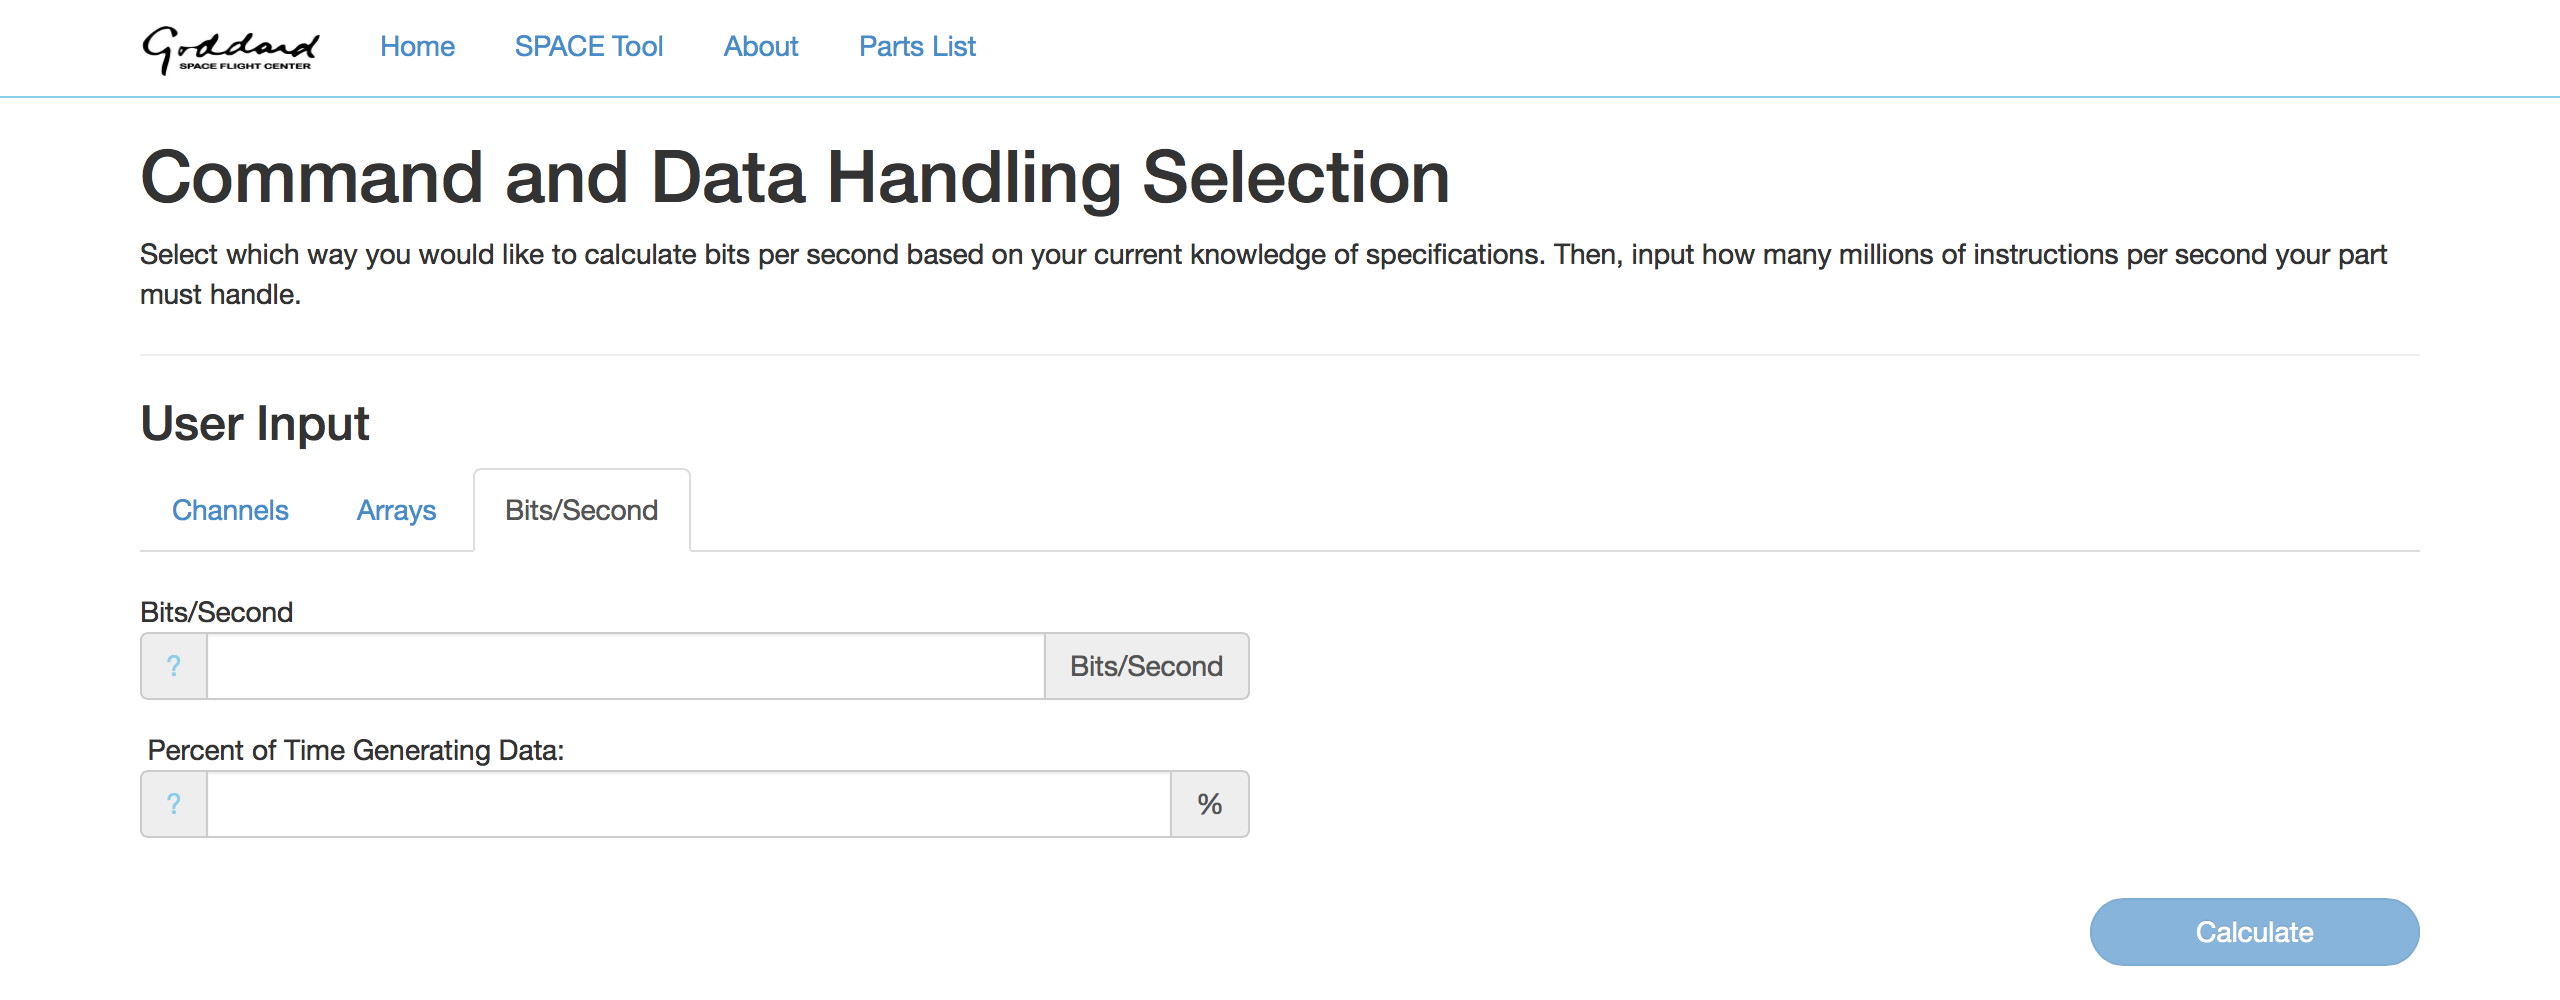
\includegraphics[width=\linewidth]{6c}
\caption{Screenshot of the CDH selection page (cont.)}
\label{default}
\end{center}
\end{figure}
This value will then be used to calculate total data volume per day by looking at the amount of time the satellite is actively generating data -- this is asked for as a percentage in a day. From there, we will display all parts with the appropriate data rate by comparing the bits per second needed for against the performance associated with the parts in the database. 
\subsection{Power Selection}
In this section, the user will be able to find an appropriate power system for their design, consisting of solar panels, batteries, and an electronic power system. The volume and a desirable configurable (deployable vs. nondeployable) will determine the applicable solar panels for your design. Following that selection, all batteries and electronic power systems will be displayed for your choosing. The power listed in this section is meant to be the power the subsystem is able to generate. In the final results page, when we are tallying the total power requirements needed by the CubeSat, we will subtract the power generated from this page. The optimal case is to end up with an overall negative power requirements, indicating that we are generating more power than we are using. 
\begin{figure}[H]
\begin{center}
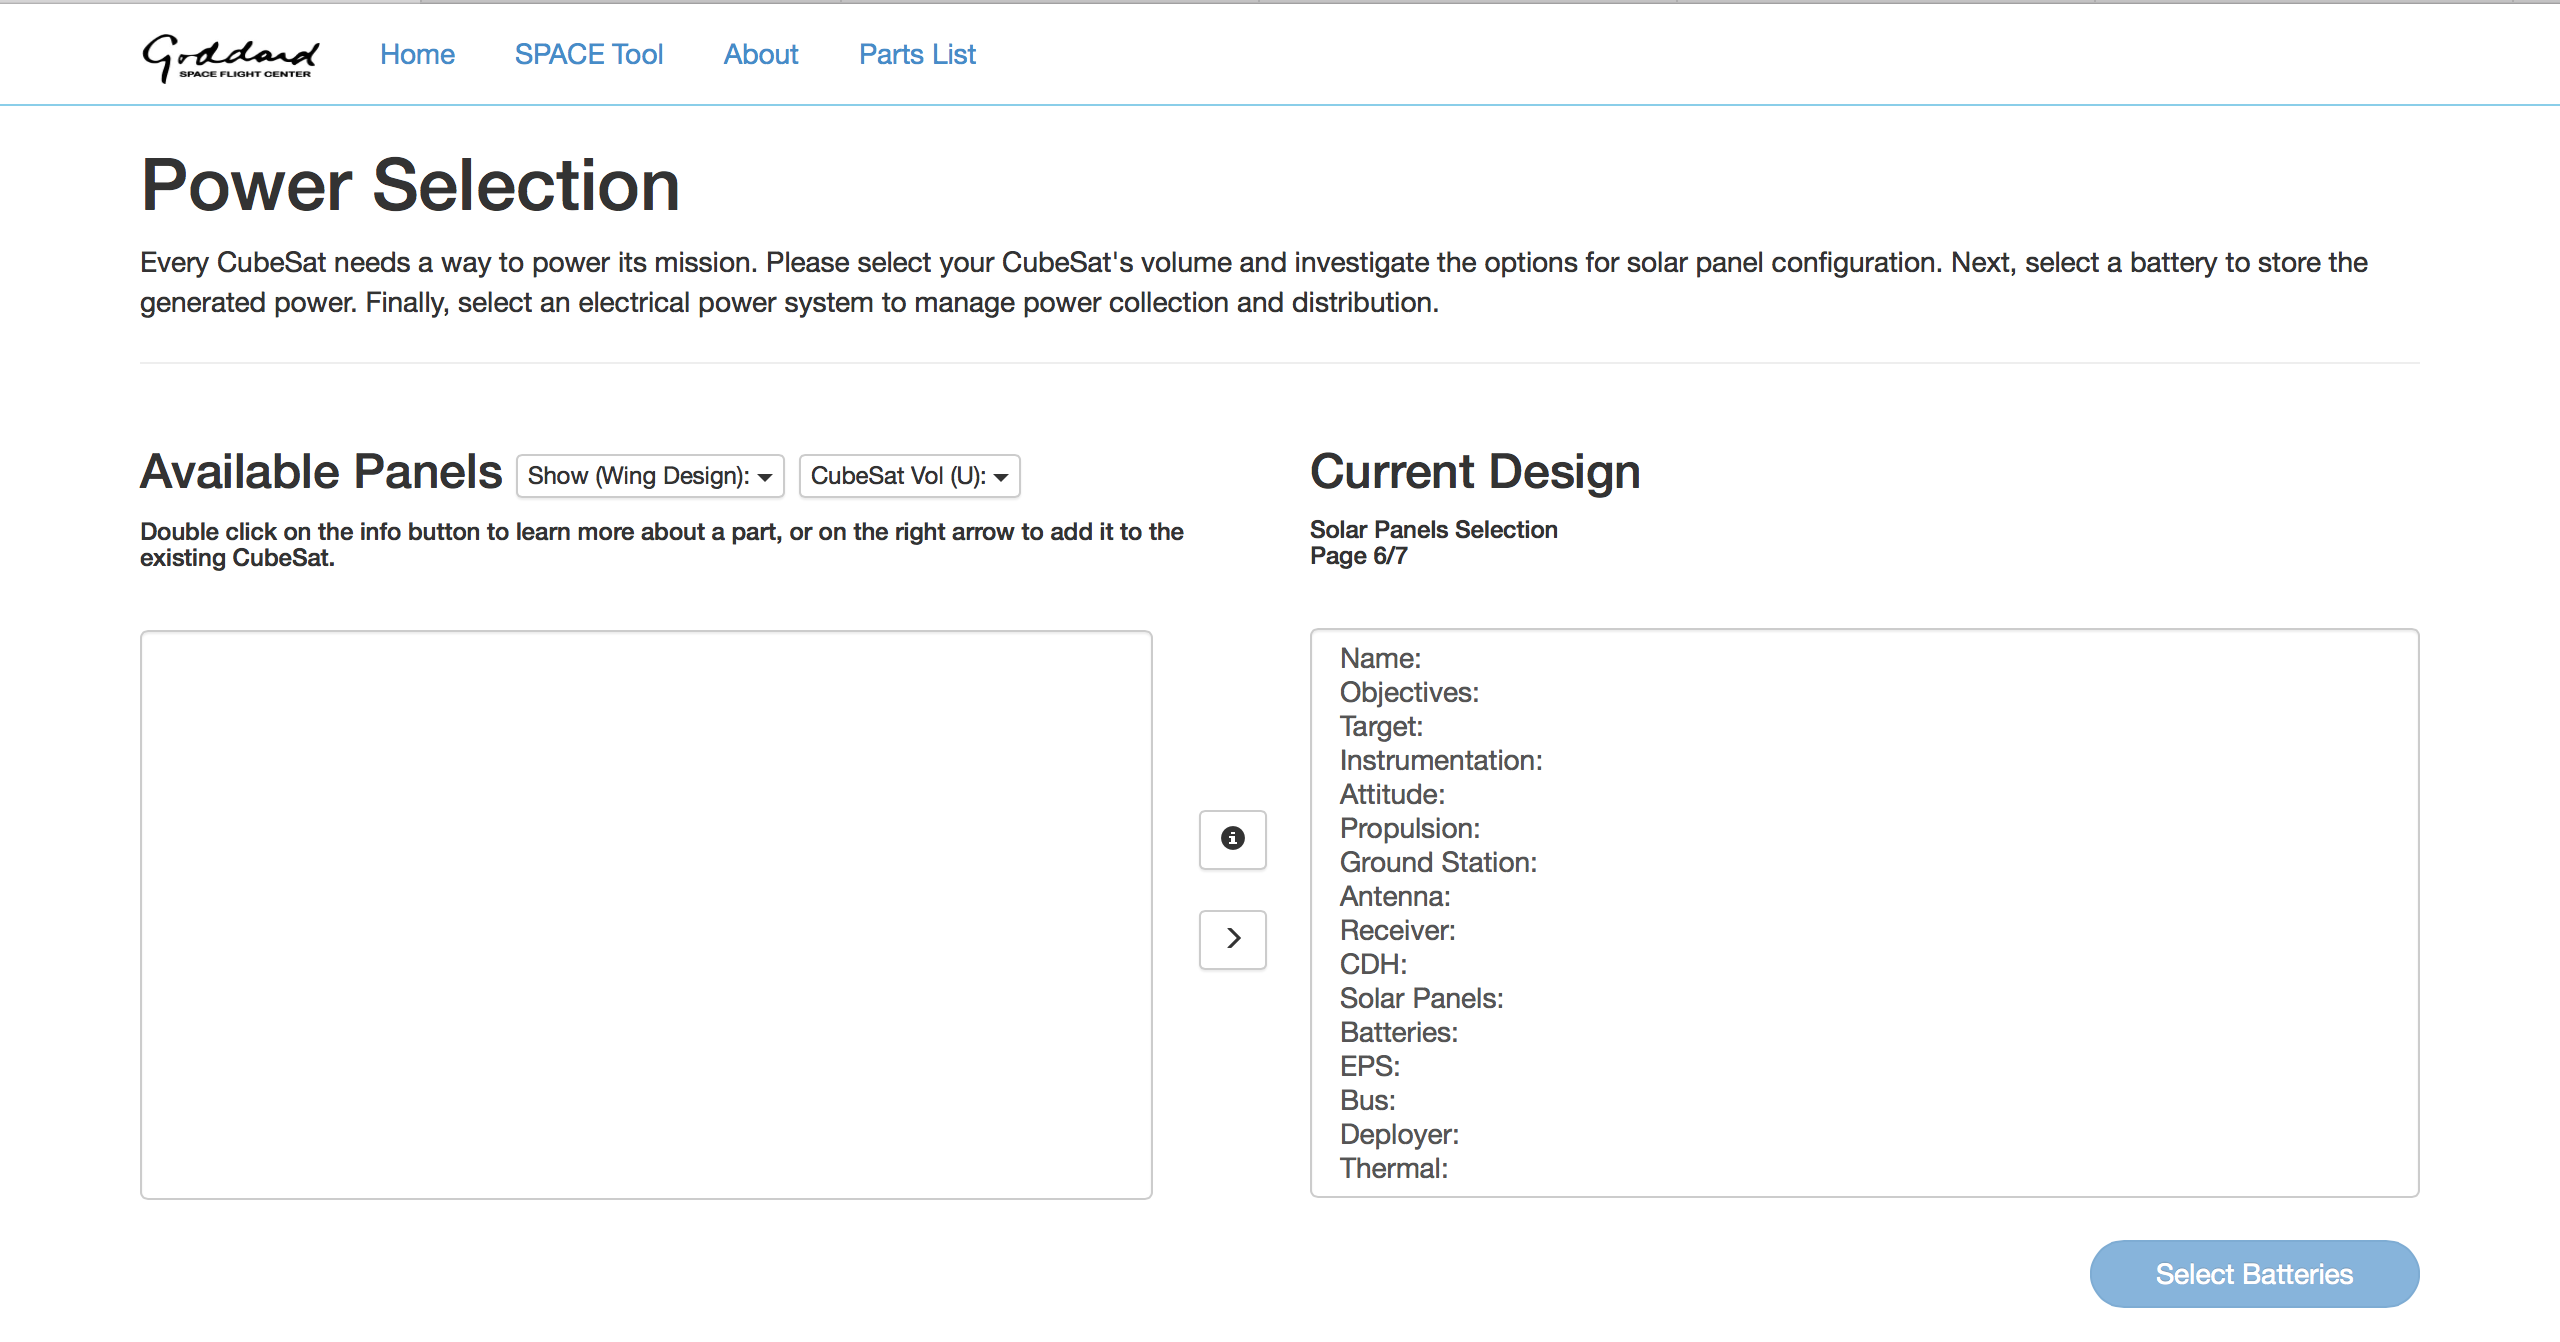
\includegraphics[width=\linewidth]{7}
\caption{Screenshot of the power selection page (cont.)}
\label{default}
\end{center}
\end{figure}
\subsection{Frame Selection}
For the final step of the CubeSat design, the user will be guided to choose a frame, deployer, and thermal system for your design. Again, these choices are dependent on the desired volume of your CubeSat design. Once that volume is chosen, all available parts matching that description will be shown. This section is also one we wish to improve with further iterations to our tool, as it is quite sparse and does not really take into account a good methodology for thermal design. 
\begin{figure}[H]
\begin{center}
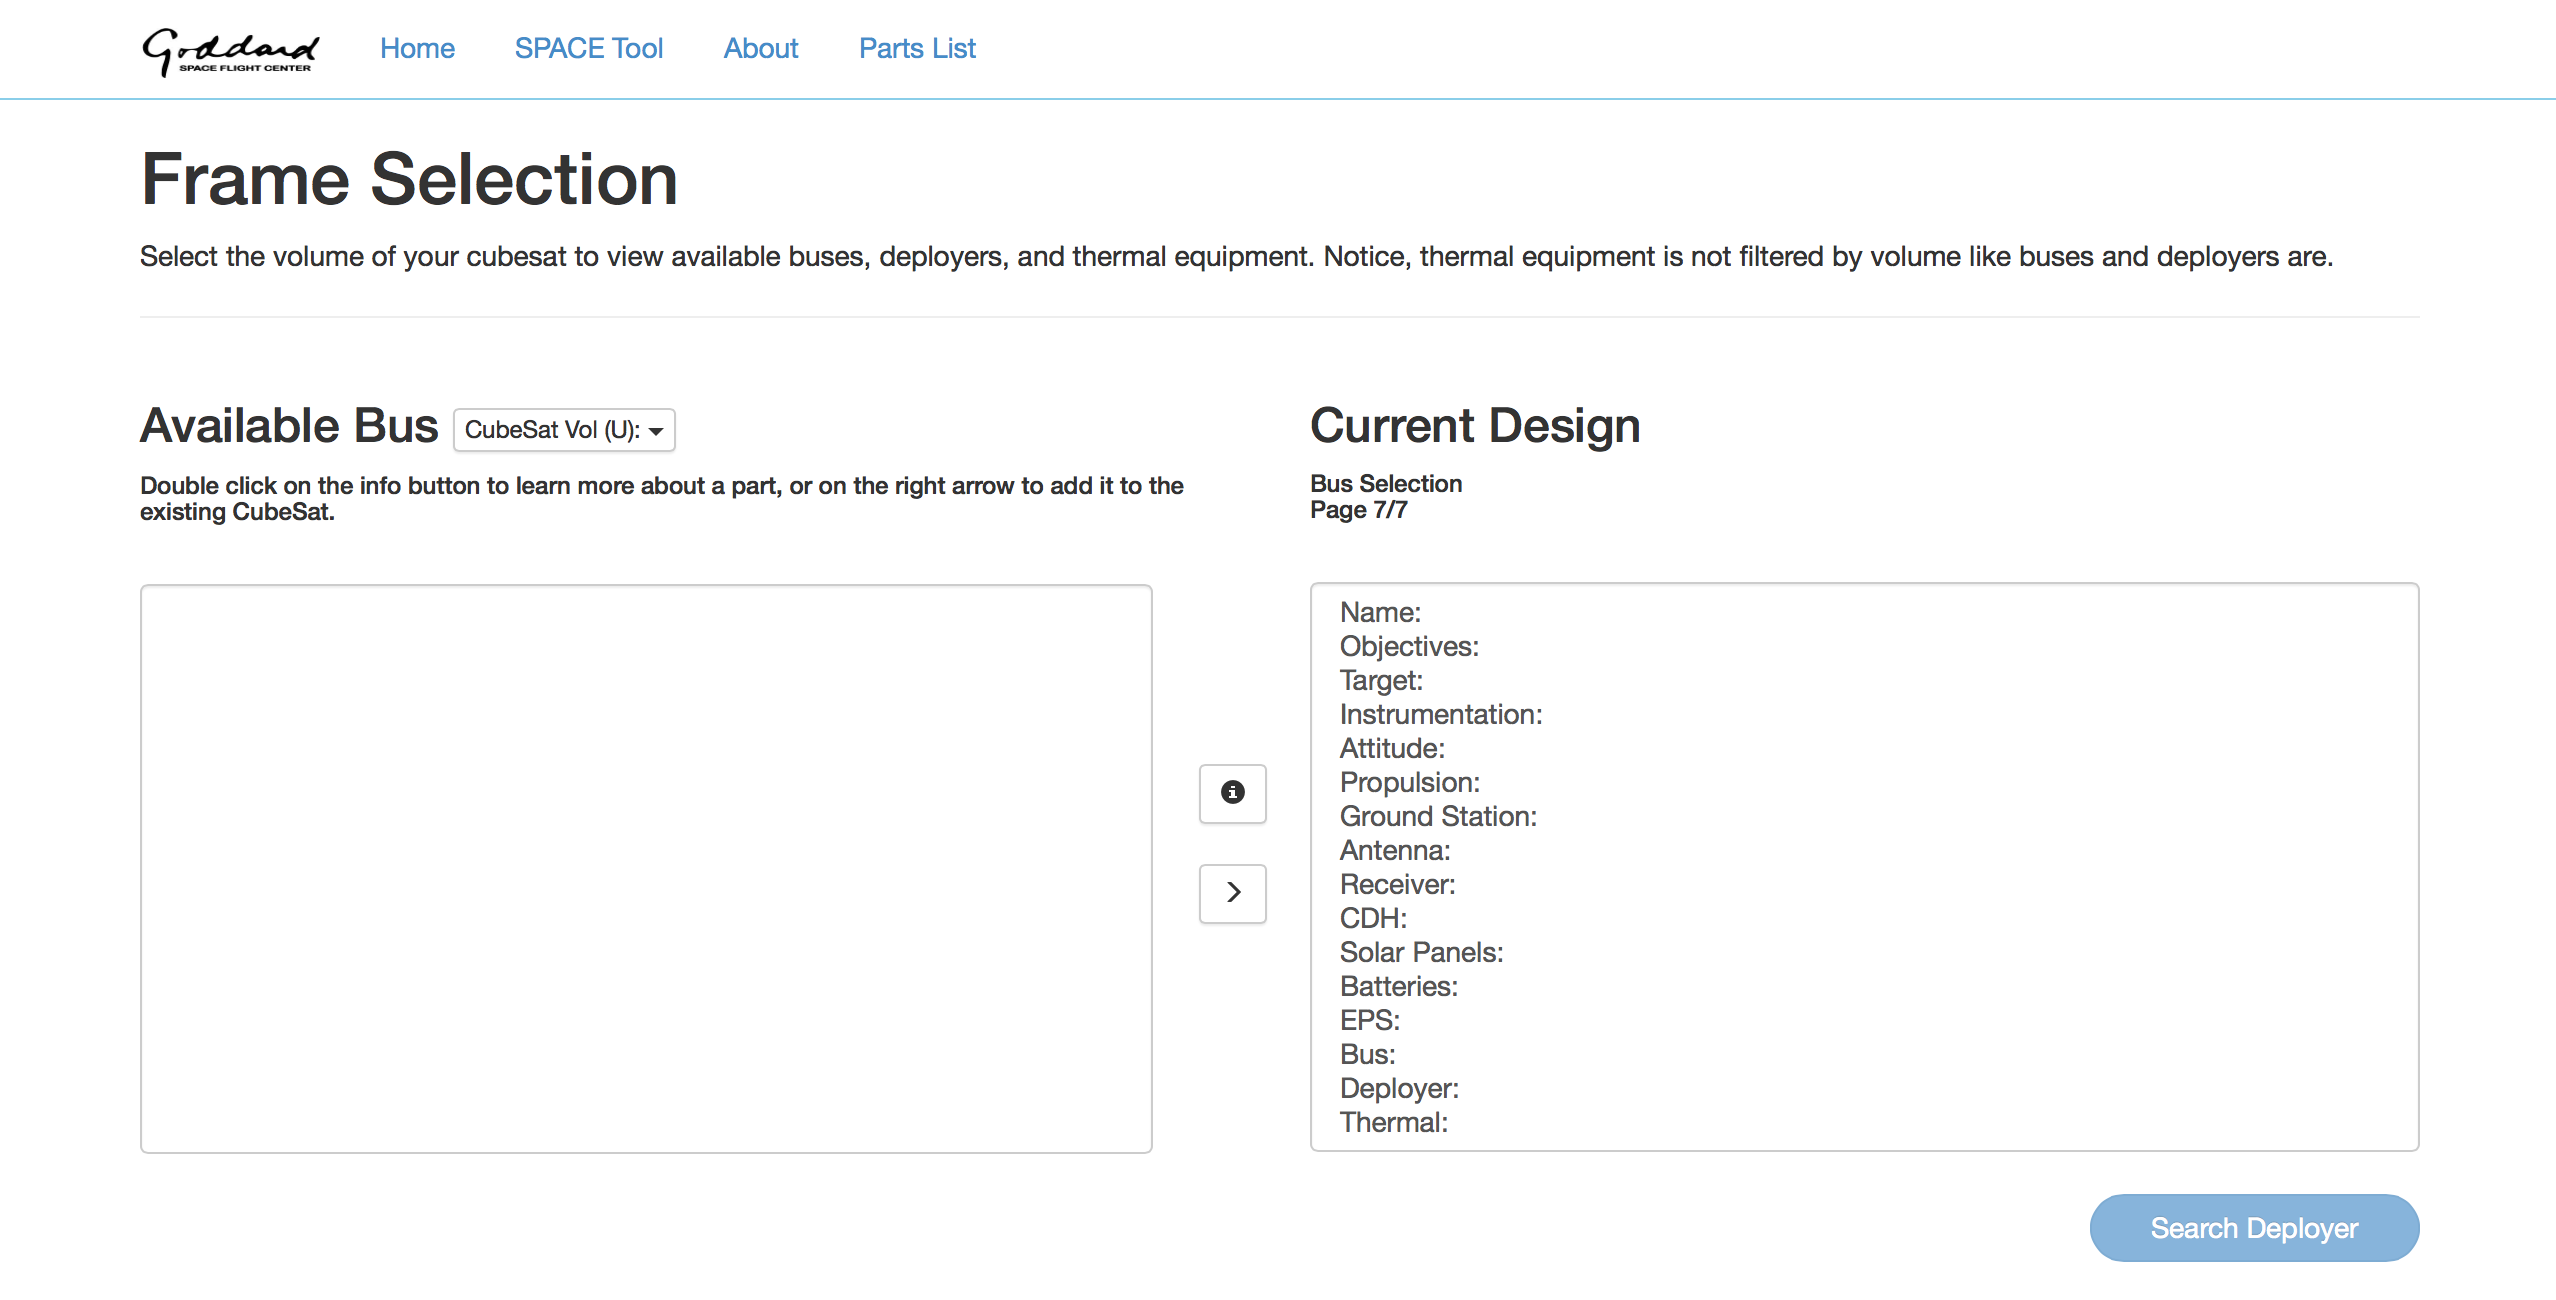
\includegraphics[width=\linewidth]{8}
\caption{Screenshot of the frame selection page (cont.)}
\label{default}
\end{center}
\end{figure}
\subsection{Final Result Page}
In the final result page, we layout the CubeSat design the user has been walked through, by displaying all the parts they have chosen, as well as the final power requirements, mass, and volume. Each subpart has an individual mass, power, and volume, as well as a link to where they can do some more research on the part. The user can print this page out through their browser. 
\begin{figure}[H]
\begin{center}
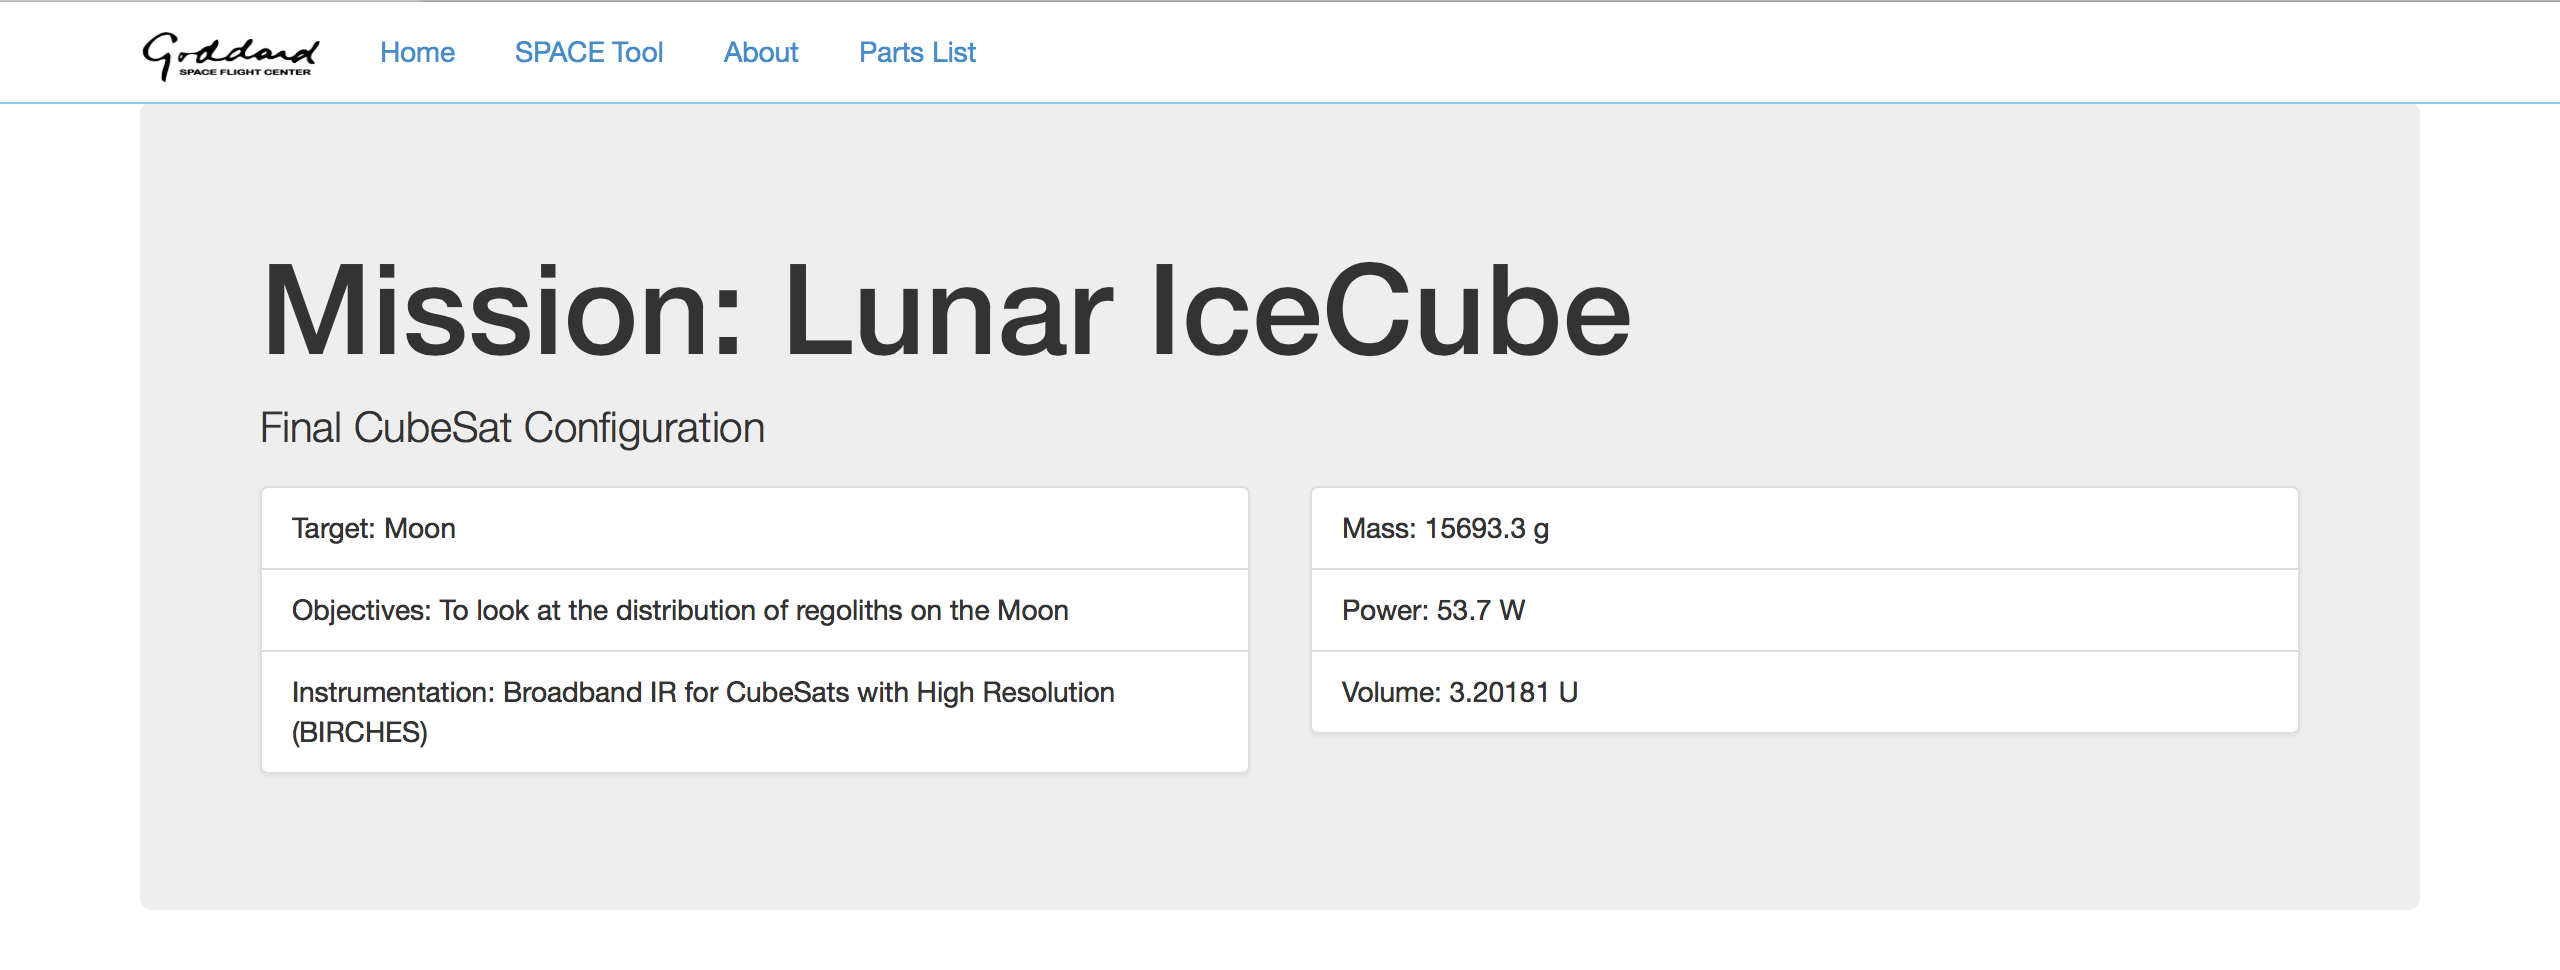
\includegraphics[width=\linewidth]{9}
\caption{Example of a mission created using this tool}
\label{default}
\end{center}
\end{figure}
\begin{figure}[H]
\begin{center}
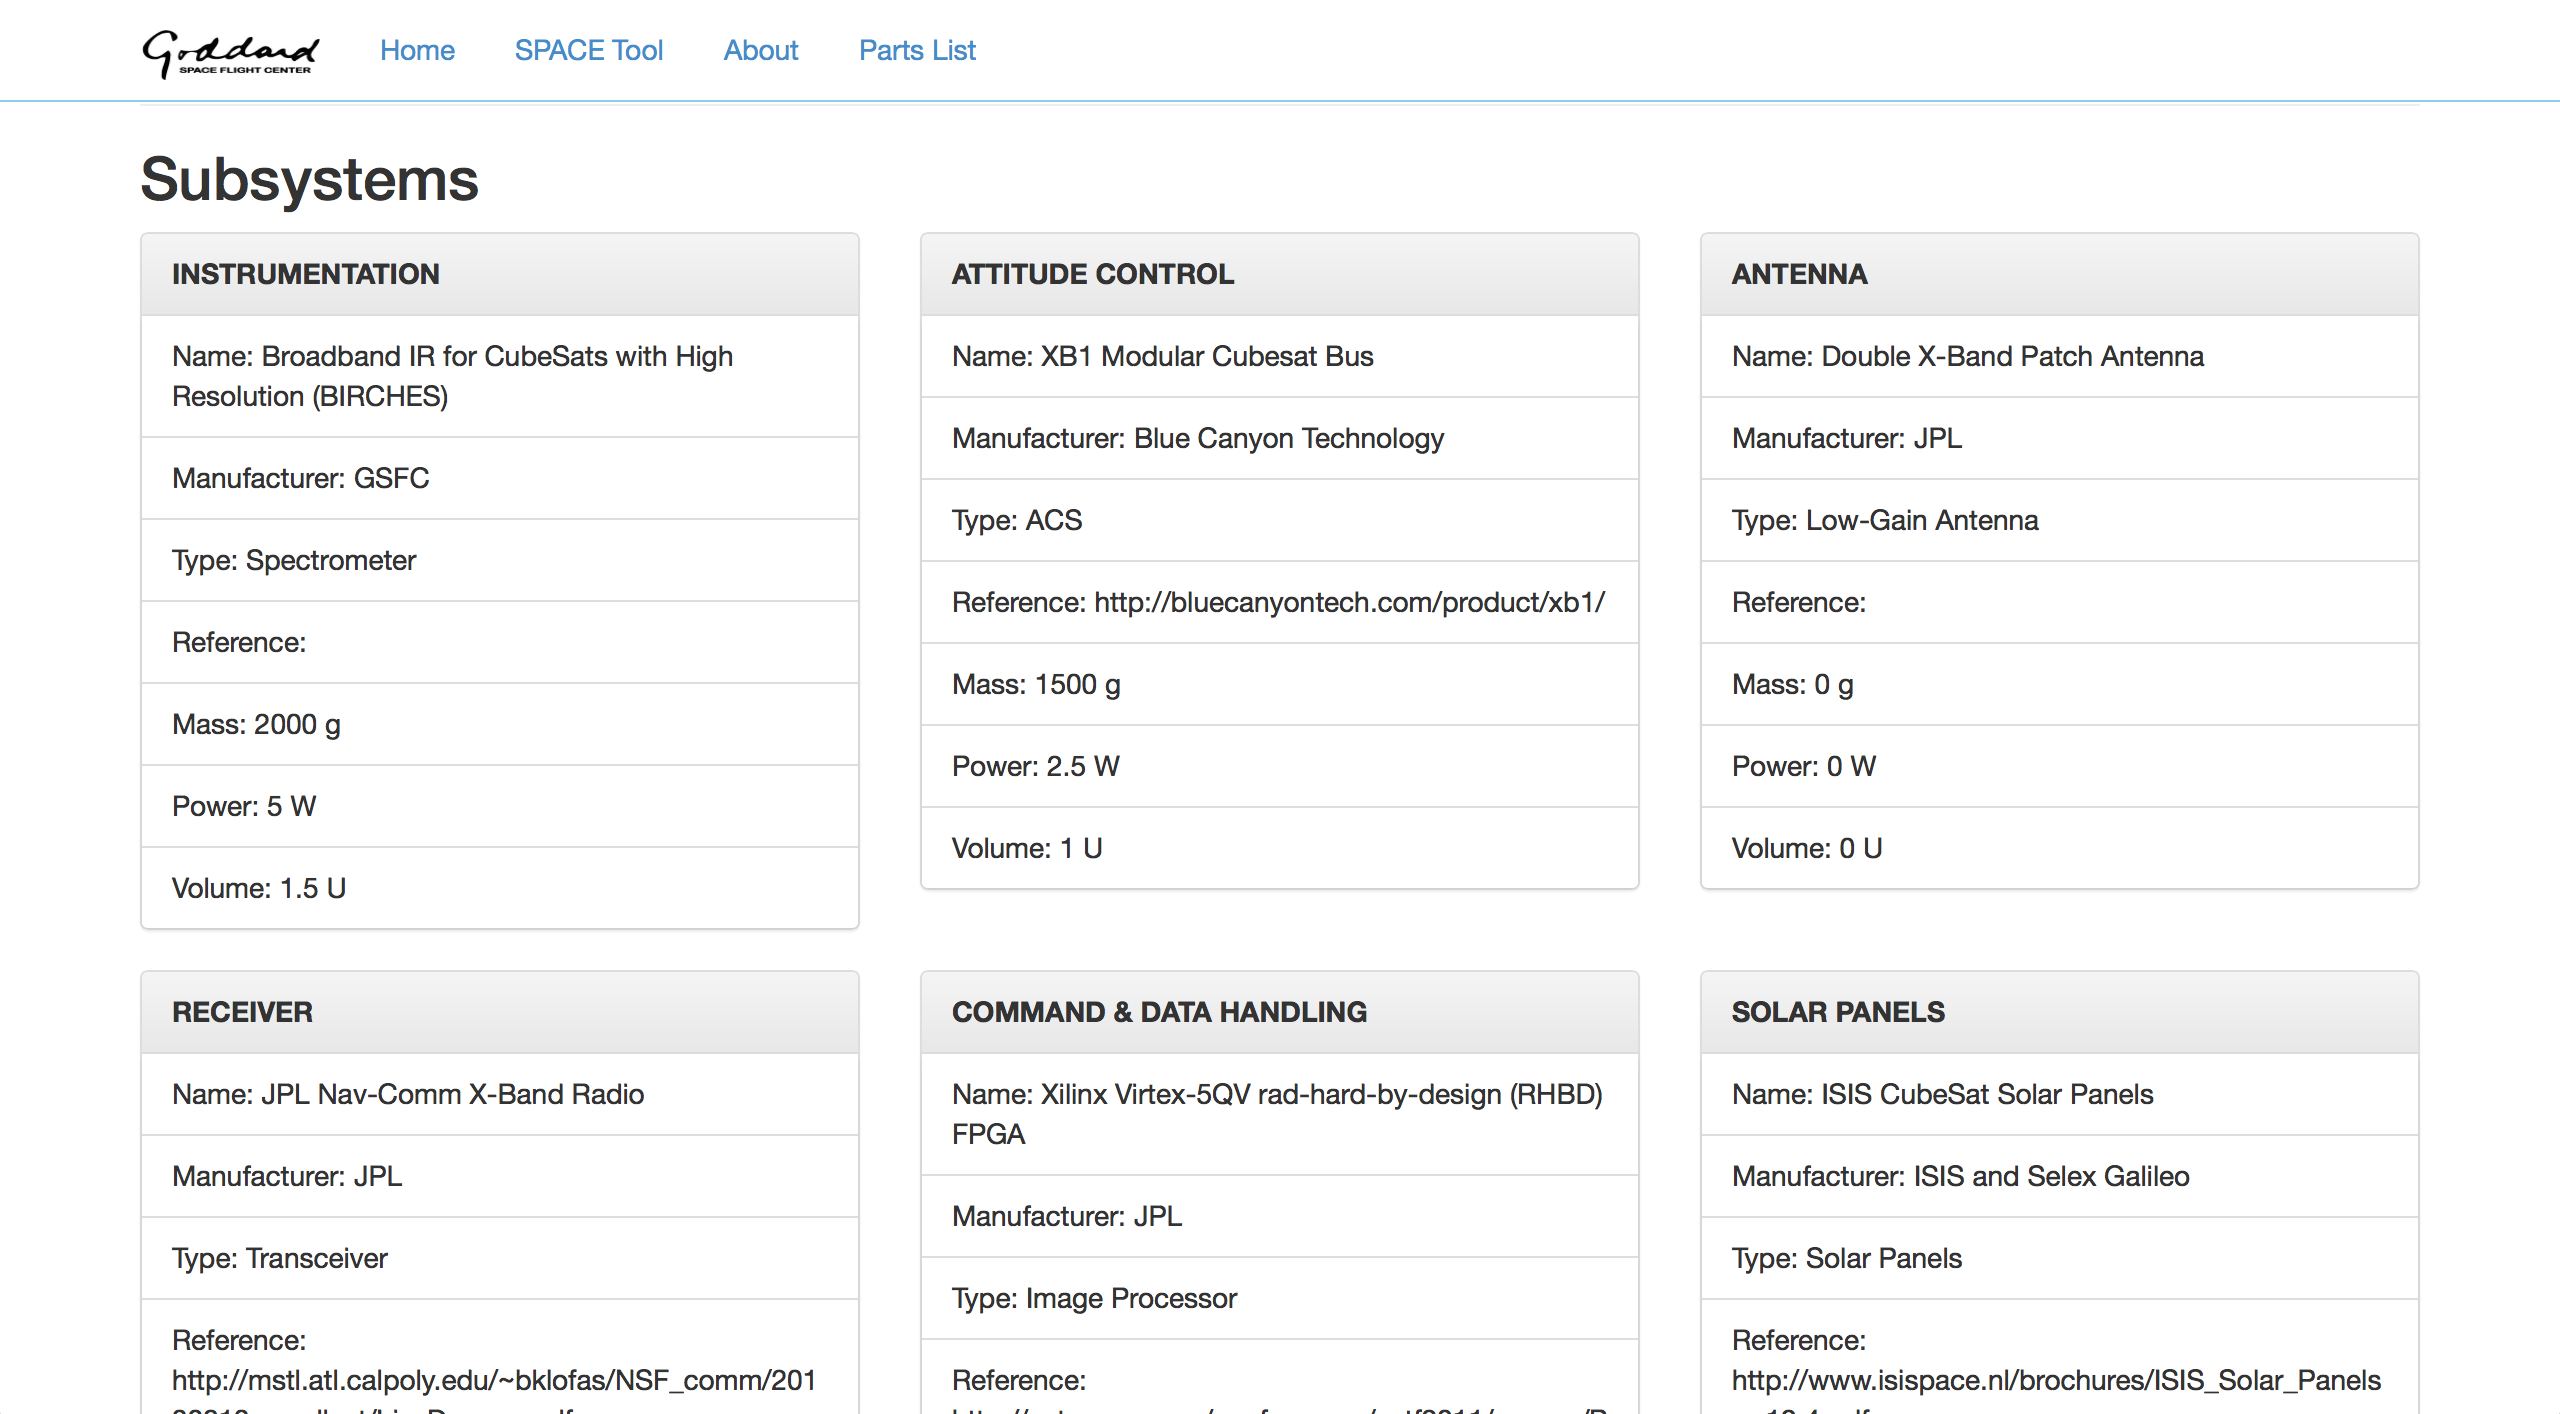
\includegraphics[width=\linewidth]{10}
\caption{Example of a mission created using this tool (cont.)}
\label{default}
\end{center}
\end{figure}
\subsection{Inputs/Output Summary}
Here we will present a concise summary of the required user inputs, and program outputs of all subpages.
\begin{table}[H]
\caption{default}
\begin{center}
\begin{tabular}{|c|c|c|c|c|}
\hline
Page & Input (s) & Unit& Output (s) & Unit\\
\hline
Instrumentation & Part of the EM Spectrum & & & \\
\hline
Attitude Control & Altitude&km & Angle of knowledge& rad\\
 &Spatial Resolution &m &Angle of control & rad\\
\hline
Trajectory Control & Direct/Indirect  & &Total $\Delta$V& km/s\\
& Apoapsis  & km& & \\
& Periapsis  & km& & \\
& Inclination Change  &rad & & \\
\hline
Communication Page & Band & & Space Loss & dB \\
 & & & Receive Power &dBW\\
 & & & Signal to Noise Ratio &dB\\
 & & & Bit Rate &Kbps\\
\hline
CDH & Total Bits Generated&bits &Bits Per Second &bps\\
&Integration Interval/Second & /s &Total Data Volume & bpd\\
\hline
Power & Volume &U & & \\
\hline
Frame & Volume& U& &  \\
\hline
\end{tabular}
\end{center}
\label{default}
\end{table}%

\section{IMPLEMENTATION}
In this section, we will talk about the design process of our webpage and the tools/frameworks used. We built the website using the MEAN stack -- utilizing Javascript for the front end, as well as the back end. The MEAN stack consists of:
\begin{enumerate}
\item MongoDB -  leading NoSQL database.
\item Express - minimal and flexible node.js web application framework.
\item AngularJS - extend HTML vocabulary for your application. 
\item Node.JS - platform built on Chrome's JavaScript runtime for easily building fast, scalable network application.\end{enumerate}
We also used Bootstrap, a front-end framework for faster and easier web development. We are hosting the database on a remote Mongolab server, and the website on an Amazon Web Services EC2 cluster. The mechanism of editing the CubeSat relies on a RESTful based architecture, through an HTTP protocol. When the user starts the tool, a POST request is sent to our CubeSat database -- this ensures all users are getting a new object to work with. This new CubeSat's object ID is saved and concatenated into the page's URL, so we can have constant access to the CubeSat the user is working on as they move on to new webpages. When each page is created, the backend Javascript makes a GET request to each subsystem's database, as well as to the object ID saved within the URL to get a copy of the current CubeSat. When we are adding parts to the current CubeSat, a PUT request is sent to the same object ID, and we can add in each subsystem as the user walks through the tool.\\[2mm]
In regards to the data, though we are using MongoDB which traditionally uses a dynamic schema, making it much more flexible, we are also using Mongoose, a wrapper that imposes a more structured format on our data in the form of schemas and types in order to ensure a more organized database.  
\section{NEXT STEPS}
This tool is actually a second generation iteration of the previous summer's Java based application. We moved the platform on to the web, making it much more accessible, responsive, and easy to use. We still have more things we wish to accomplish, namely making some of the algorithms more exact and take away some of the generalities built into the tool. We are also working to make the website more secure, adding in a logging system for the database. As of now, any user can add parts to our database, which is not exactly desirable. We also want to begin modifying the architecture of schemas for the CubeSat, in order to make it possible for two parts of the same subsystem to be able to be added to the CubeSat -- such as two instruments, or two propulsion systems. Last, one thing that we are always working on improving is our database, making it more standardized and adding parts that are current technology innovations.
\newpage
\section{REFERENCES}
[1] ``Bootstrap - The world's most popular mobile-first and responsive front-end framework.,'' \textit{Bootstrap - The world's most popular mobile-first and responsive front-end framework}. [Online]. Available at: http://getbootstrap.com. [Accessed: 2015].\\[2mm]

\noindent [2] P. E. Clark and M. L. Rilee, \textit{Remote sensing tools for exploration observing and interpreting the electromagnetic spectrum}. New York: Springer, 2010.\\[2mm]

\noindent [3] ``MEAN - Full-Stack JavaScript Using MongoDB, Express, AngularJS, and Node.js.,'' \textit{MEAN.IO}. [Online]. Available at: http://mean.io/. [Accessed: 2015].\\[2mm]

\noindent [4] ``Propagation Tutorial - Link Budgets.,'' \textit{Propagation Tutorial - Link Budgets.} [Online]. Available at: http://www.mike-willis.com/tutorial/pf13.htm. [Accessed: 2015].\\[2mm]

\noindent [5] ``Radar Basics.,'' \textit{Free-Space Path Loss.} [Online]. Available at: http://www.radartutorial.\\eu/01.basics/free-space path loss.en.html. [Accessed: 2015].\\[2mm]

\noindent [6] ``Radio Frequencies for Space Communication.,'' \textit{Radio Frequencies for Space Communication.} [Online]. Available at: http://www.spaceacademy.net.au/spacelink/radiospace.htm. [Accessed: 2015].\\[2mm]
\section{CONTACT US}
(Mentor) Pamela E. Clark - NASA Jet Propulsion Laboratory --- pamela.e.clark@jpl.nasa.gov\\[3mm]
Huong Vo - University of Washington --- huongnvo@uw.edu \\[3mm]
Aparna Natarajan - University of Maryland, College Park --- aparnan09@gmail.com\\[3mm]
Zoe Himwich - Stanford University --- zoeh917@gmail.com

\end{document}
